\documentclass{bmcart}

\usepackage{xcolor}
\usepackage{url}
\usepackage{amsmath}
\usepackage{amsthm}
\usepackage{amssymb}
\usepackage{graphicx}
\usepackage{tikz}
\usetikzlibrary{shapes,arrows}
\usepackage{float}
\usepackage{verbatim}
\usepackage{tabu}
\usepackage{multirow}
\usepackage{framed}
\usepackage{xr}
\externaldocument{supplement}

\usepackage{verbatim}
\usepackage{gensymb}
\usepackage{listings}

\usepackage{soul}

\newcommand{\beginsupplement}{%
        \setcounter{table}{0}
        \renewcommand{\thetable}{S\arabic{table}}%
        \setcounter{figure}{0}
        \renewcommand{\thefigure}{S\arabic{figure}}%
     }

\newcommand{\pname}[1]{\texttt{ChIPexoQual}}
\newcommand{\SK}[1]{\textcolor{red}{SK: #1}}
\newcommand{\RW}[1]{\textcolor{blue}{RW: #1}}

% \usepackage{authblk}
\usepackage[utf8]{inputenc} %unicode support

\newcommand{\sig}{\sigma^{70}}

\begin{document}

\begin{frontmatter}

\begin{fmbox}
\dochead{Research}

\title{Data Exploration, Quality Control, and Statistical Analysis of
  ChIP-exo/nexus Experiments}

\author[
   addressref={aff1},
   noteref={n1},
   email={welch@stat.wisc.edu}      
]{\inits{RW}\fnm{Rene} \snm{Welch} }
\author[
   addressref={aff6},        % id's of addresses, e.g. {aff1,aff2}
   noteref={n1},
   email={chungd@musc.edu}   % email address
]{\inits{DC}\fnm{Dongjun} \snm{Chung} } 
\author[
   addressref={aff3,aff4},
   email={jagrass@wisc.edu}
]{\inits{JG}\fnm{Jeffrey} \snm{Grass}}
\author[
   addressref={aff3,aff4,aff5},
   email={landick@bact.wisc.edu}
]{\inits{RL}\fnm{Robert} \snm{Landick}}
\author[
   addressref={aff1,aff2},
   corref={aff1},
   email={keles@stat.wisc.edu}
]{\inits{SK}\fnm{S\"und\"uz} \snm{Kele\c{s}}}

\address[id=aff1]{%                           % unique id
  \orgname{Department of Statistics, University of Wisconsin Madison}, % university, etc
  \street{1300 University Avenue},                     %
  %\postcode{}                                % post or zip code
  \city{Madison},                              % city
  \cny{WI}                                    % country
}

\address[id=aff2]{%
  \orgname{Department of Biostatistics and Medical Informatics, University of Wisconsin Madison},
  \street{600 Highland Avenue},
%  \postcode{24105}
  \city{Madison},
  \cny{WI}
}
\address[id=aff3]{
  \orgname{Great Lakes Bioenergy Research Center, University of Wisconsin Madison},
  \street{1552 University Avenue},
  \city{Madison},
  \cny{WI}
}
\address[id=aff4]{
  \orgname{Department of Biochemistry, University of Wisconsin Madison},
  \street{433 Babcock Drive},
  \city{Madison},
  \cny{WI}
}
\address[id=aff5]{
  \orgname{Department of Bacteriology, University of Wisconsin Madison},
  \street{1550 Linden Drive},
  \city{Madison},
  \cny{WI}
}
\address[id=aff6]{
  \orgname{Department of Public Health Sciences, Medical University of South Carolina},
  \street{135 Cannon Street},
  \city{Charleston},
  \cny{SC}
}

\begin{artnotes}
\note[id=n1]{These two authors contributed equally.} % note, connected to author
\end{artnotes}


\end{fmbox}

\begin{abstractbox}

\begin{abstract}
ChIP-exo/nexus experiments present modifications on the commonly used ChIP-seq protocol for high resolution mapping of transcription factor binding sites. Although many aspects of the ChIP-exo data analysis are similar to those of ChIP-seq, these high throughput experiments pose a number of unique quality control and analysis challenges. We develop a statistical quality control pipeline and accompanying \texttt{R} package, \pname{}, to enable exploration and analysis of ChIP-exo and related experiments. \pname{} evaluates a number of key issues including strand imbalance, library complexity, and signal enrichment of data. Assessment of these features are facilitated through diagnostic plots and summary statistics calculated over regions of the genome with varying levels of coverage.
    
We evaluated our QC pipeline with both large collections of public ChIP-exo/nexus data and multiple, new ChIP-exo datasets from \textit{E. Coli}. \pname{} analysis of these datasets resulted in guidelines for using these QC metrics across a wide range of sequencing depths and further insights for modelling ChIP-exo data.Finally, although ChIP-exo experiments have been compared to ChIP-seq experiments with single-end (SE) sequencing, we provide, for the first time, comparisons with paired-end (PE) ChIP-seq experiments. We illustrate that, at fixed sequencing depths, ChIP-exo provides higher sensitivity, specificity, and spatial resolution than PE ChIP-seq and both significantly outperform their SE ChIP-seq counterpart. Furthermore, we show that for binding events separated by 200-400 bp ChIP-exo exhibits a significantly higher sensitivity.

%    \SK{The last sentence does not really make much sense? }, \RW{I
%      meant that when we have a peak composed by more than one binding
%      event, as the mean distance between binding events increases
%      then ChIP-exo is more likely to identify all the binding events,
%      I used sensitivity because we defined it as the proportion of
%      identified binding events in a given peak. I think it depends if
%      we decide to add Fig8 in the main article or in the
%      supplement.}
      
%\pname pipeline explores and quantifies these aspects by partitioning the experiment reads into a collection of regions, calculating a series of summary statistics for each region, providing visualizations and calculating measures to globally asses t quality of a ChIP-exo experiment. 
%In addition, we demonstrate that the ChIP-exo QC pipeline it is also applicable to ChIP-nexus data, showing that those experiments present higher quality than ChIP-exo experiments under similar conditions.
%We compared ChIP-exo with Paired End (PE) and Single End (SE) ChIP-Seq and found the following characteristics: First, although often assumed in ChIP-exo data analysis methods, the ``peak pair'' assumptions does not hold locally in actual ChIP-exo data. Second, we for the first time compared PE ChIP-Seq with ChIP-exo and found that 

% ChIP-exo and PE ChIP-seq are comparable in sensitivity for closely located binding events, but as the average distance between binding events increases, ChIP-exo exhibits higher sensitivity than PE ChIP-seq.      
\end{abstract}

\begin{keyword}
\kwd{ChIP-exo}
\kwd{ChIP-nexus}
\kwd{ChIP-seq}
\kwd{Statistical Quality Control}
\kwd{Spatial Resolution}
\kwd{Transcription Factor}  
\kwd{Deconvolution}
\kwd{Binding Site Identification with High-Resolution.}
\end{keyword}

\end{abstractbox}

\end{frontmatter}

\newpage

\section*{Background}
\label{sec:intro}

Chromatin Immunoprecipitation followed by exonuclease digestion and next generation sequencing (ChIP-exo) is currently one of the state-of-the-art high throughput assays for profiling protein-DNA interactions at or close to single base-pair resolution \cite{exo1}. It presents a powerful alternative to popular ChIP-seq (Chromatin Immunoprecipitation coupled with next generation sequencing) assay. ChIP-exo experiments first capture millions of DNA fragments ($150$ - $250$ bps in length) that the protein under study interacts with using a protein-specific antibody and random fragmentation of DNA. Then, $\lambda$-exonuclease ($\lambda$-exo) is deployed to trim the $5^{\prime}$ end of each DNA fragment to each protein-DNA interaction boundary. This step is unique to ChIP-exo and aims to achieve significantly higher spatial resolution compared to ChIP-seq. Finally, high throughput sequencing of a small region ($36$ to $100$ bps) at the $5^{\prime}$ end of each fragment generates millions of reads. Similarly, ChIP-nexus (Chromatin Immunoprecipitation followed by exonuclease digestion, unique barcode, single ligation and next generation ligation) \cite{chipnexus} is a further modification on the ChIP-exo protocol. ChIP-nexus aims to overcome limitations of ChIP-exo by yielding high complexity libraries with numbers of cells comparable to that of ChIP-seq experiments. This is achieved by reducing the numbers of ligations in the standard ChIP-exo protocol from two to one, and adding unique, randomized barcodes to adaptors to enable monitoring of overamplification. Figure~\ref{fig:1}A illustrates the differences between different ChIP-based protocols: ChIP-exo, single-end (SE) ChIP-seq, paired-end (PE) ChIP-seq, ChIP-nexus. The $5^{\prime}$ ends of a ChIP-exo/nexus experiment are clustered more tightly around the binding sites of the protein than in a ChIP-seq experiment. In a PE ChIP-seq experiment, both ends are sequenced as opposed to only the $5^{\prime}$ end in a SE ChIP-seq.

% \RW{This modification makes a library generated using the ChIP-nexus protocol to be larger than one generated with ChIP-exo, which where both sequencing adaptors are ligated at the end of the ChIP fragments. Then, after exonuclease digestion, DNA self-circularization with circLigase, and restriction enzyme cutting between the two adaptors, the final library is amplified. Compared to ChIP-exo, ChIP-nexus aims to   attain  higher resolution analysis while yielding higher complexity libraries.

% \SK{Note to Rene: ChIP-nexus paper has a good description of what can go wrong with ChIP-exo; It seems like most of the read imbalance could also be due to ligation inefficiency. Although this probably does not explain why we have reads only from one strand in some regions. This is more likely explained by over digestion in one strand or single stranded TF-DNA interaction. Think a bit more on these issues and understand how the ligation could give rise to strand imbalance, we can ask Bob to have a closer look at the section where we have this discussion.}

% \RW{1 - I think it may come from the starting material in each side. I think that at least the number of fragments on each side must preserve that if there is more starting reads in one side, then this must be the case after the amplification.} 
% \RW{2 - There is not control about how the enzyme digests the fragments, as far as we know it starts on the $5\prime$ side and stops until it finds the TF or it runs out of energy to keep digesting. I think Bob mentioned that it may be possible for the enzyme to pass though the TF if it is left digesting for a longer time, but if that's the case then the question may be why it preffers one strand over the other, which may lead to the GC-bias but as far as I can tell is very hard to observe that because that bias appear also in ChIP-seq (and it seeems that also appear in the circularization step from ChIP-nexus).}

% \RW{3 - I think that the regions formed by fragments in one strand, may be copies of few undigested fragments, in a good experiment the    fragments are expected to be clustered around the binding sites, therefore it is less likely to observe this fragments scattered in the genome. In a bad experiment is the opposite case, so the fragments are not clustered so if the enzyme doesn't have a strong preference to how is attracted to the fragments then the remaining ones can be seen as random positions around the genome, this positions are copied several times during the amplification and that may be the reason why we observe something as scattered. Perhaps if the enzyme was left for longer time, then the starting material that later was amplified into this regions would have been digested and some of this regions wouldn't appear (I am thinking about the deeply sequenced TBP experiments.)}

Although ChIP-exo/nexus protocols are being adopted by research community, features of ChIP-exo data, especially those pertaining to data quality, have not been investigated much. The key features of ChIP-exo/nexus that separate them from ChIP-seq are broadly as follows. First, DNA libraries generated by the ChIP-exo protocol are expected to be less complex than the libraries generated by ChIP-seq \cite{exo_review}) because digestion by $\lambda$-exo is expected to restrict the space of genomic positions that sequencing reads can map to, to small local regions around the actual binding sites. Therefore, in high quality and especially deeply sequenced ChIP-exo datasets, it is possible to observe large numbers of reads accumulating at a small number of bases due to actual signal rather than overamplification bias as commonly observed in ChIP-seq experiments.  Second, although we expect approximately the same numbers of reads from both DNA strands at a given binding site, there may be locally more reads in one strand than in the other, owing to $\lambda$-exo efficiency, ligation efficiency, or other factors. This is a key point with implications on the statistical analysis of ChIP-exo data. Specifically, currently available ChIP-exo specific statistical analysis methods (e.g., Mace \cite{mace}, CexoR \cite{cexor}, and Peakzilla \cite{peakzilla}) rely on the existence of peak-pairs formed by forward and reverse strand reads at the binding site. Finally, most of current widely used ChIP-seq quality control (QC) guidelines \cite{encode_qc} may not be directly applicable to ChIP-exo data.

To address these challenges, we develop a suite of diagnostic plots and summary statistics and implement them in a versatile \texttt{R ackage} named \pname{}.  We apply this pipeline on a large collection of public and newly generated ChIP-exo/nexus data. We validate the QC pipeline by evaluation of the samples for features that capture high signal to noise such as occurrences of motifs recognized by the profiled DNA interacting protein. Our analyses of this large collection of data reveal that the ChIP-exo peak-pair assumption, underlying most of the ChIP-exo analysis pipelines is subject to violations. To further address this and provide a platform where ChIP-exo and ChIP-seq experiments can be evaluated with comparable methods, we assess performances of recently developed methods suitable for ChIP-exo analysis, including dPeak \cite{dpeak} and GEM \cite{gem}. We observe that dPeak performs as good or better than the available ChIP-exo methods and provides a platform where PE and SE ChIP-seq can be compared with their ChIP-exo counterpart. Our comparisons of PE ChIP-seq with ChIP-exo interestingly highlights that while ChIP-exo outperforms PE ChIP-seq in terms of resolution and detection power, both are significantly better than SE ChIP-seq.

% while there are not established QC pipelines for ChIP-exo; previous ChIP-exo analyses used ChIP-Seq samples to compare the resolution  between experiments \cite{exo1,exoillumina,exo2}.

%to interrogate these biases in a ChIP-exo experiment and globally asses the enrichment and library complexity of a ChIP-exo sample and a procedure to distinguish low complexity libraries from deeply sequenced experiments. This aspect is unique to ChIP-exo, since the exonuclease enzyme it is expected to digested the reads that are not bound to a transcription factor, therefore the number of bases where a ChIP-exo fragment could be potentially aligned is reduced. That way, in a high quality ChIP-exo experiment is possible to observe a large amount of reads to be aligned to unique position due to genomic signal instead of PCR artifacts.

%In order to obtain the potential benefits of ChIP-exo on protein binding site identification, it is critical to use algorithms that could fully utilize information available in ChIP-exo data. Rhee and Pugh, 2011 \nocite{exo1} discussed that reads in the forward and reverse strand might construct peak pairs around bound proteins, of which heights were implicitly assumed to be symmetric. Based on this rationale, they used the ``peak pair method'' that predicts the midpoint of two modes of peak pairs as potential binding sites. Recently developed ChIP-exo data analysis methods, such as Mace (Wang et al, 20114\nocite{mace}), CexoR (Madrigal, 2015\nocite{cexor}) and Peakzilla (Bardet et al., 2013\nocite{peakzilla}), are also based on this peak pair assumption. However, appropriateness of such assumption was not fully evaluated in the literature yet. Furthermore, it is still unknown which factors could affect protein binding site identification using ChIP-exo data. In order to address this problem, we investigated various aspects of ChIP-exo data by contrasting them with their respective ChIP-Seq experiments.

%Currently, research on statistical methods for ChIP-exo data is still in its very early stage. Although many methods have been proposed to %identify protein binding sites from ChIP-Seq data (reviewed by Wilbanks and Facciotti, 2012\nocite{evaluation} and Pepke and Wold, 2009 \nocite{computation}), such as MACS (Zhang et al., 2008\nocite{macs}), CisGenome (Ji et al., 2008\nocite{cisgenome}) and MOSAiCS (Kuan et al., 2009\nocite{mosaics}), these approaches might not fully utilize potentials of ChIP-exo data for high resolution identification of protein binding sites. Specifically these approaches reveal protein binding sites only in lower resolution, i.e., at an interval of hundreds to thousands of base pairs. Furthermore, they implicitly assume that there is only one ``mode'' or ``predicted binding location'' per this wide genomic interval. More recently, deconvolution algorithms such as Deconvolution (Lun et al., 2009\cite{csdeconv}), GEM (Guo et al., 2012\nocite{gem}, an improved version of Guo et al., 2010\nocite{gps} ) and PICS (Zhang et al., 2010\nocite{pics}) have been proposed to identify binding sites in higher resolution using ChIP-Seq data. However, most of them are still not tailored for ChIP-exo and PE and SE ChIP-Seq data in a unified framework and as a result, currently available methods are not appropriate for fair comparison between ChIP-exo and ChIP-Seq. To address these limitations, we developed and utilized an improved version of dPeak (Chung et al., 2013\nocite{dpeak}), a high resolution binding site identification (deconvolution) algorithm that we previously developed for PE and SE ChIP-Seq data, so that it can also handle ChIP-exo data. The dPeak algorithm implements a probabilistic model that accurately describes the ChIP-exo and ChIP-Seq data generation process.

%Some of the key findings in this work are as follows. First, we demonstrate that the ``peak pair'' assumption of Rhee and Pugh, 2013\nocite{exo2} does not hold well in real ChIP-exo data. Second, we found that when analyzing ChIP-exo data and the Input control is not available, it is useful to adjust for GC content and mappability biases to improve peak calling and binding site identification. Third, we evaluated several methods to identify binding events and dPeak performs competitively respect to GEM and MACE when analyzing ChIP-exo data. Finally, when comparable number of reads is used for both ChIP-exo and ChIP-Seq , dPeak coupled with ChIP-exo data provides resolution comparable to PE ChIP-Seq and both significantly improve the resolution of protein binding identification compared to SE-based analysis with any of the available methods.

\section*{Results and discussion}
\label{sec:results}

\subsection*{Publicly available ChIP-exo/nexus and novel \textit{E. Coli} ChIP-seq/exo datasets}

We utilized a rich collection of publicly available ChIP-exo/nexus data from multiple organisms to build and evaluate our quality control pipeline (Table~\ref{tab:qc}). These include: CTCF factor in human HeLa cells \cite{exo1}; ER factor in human MCF-7 cells \cite{exoillumina}; GR factor in IMR90, K562, and U2OS human cells \cite{starick15}; TBP factor in human K562 cells \cite{venters13}. ChIP-nexus data included experiments from \cite{chipnexus} profiling TBP in human K562 cells, MyC and Max in \textit{D. melanogaster} S2 cells, and Twist and Dorsal in \textit{D. melanogaster} embryo.

In order to have a setting where we can compare SE and PE ChIP-seq with their ChIP-exo counterpart, we profiled $\sig$ under a variety of conditions in \textit{E. coli} with both ChIP-exo and PE ChIP-seq (Table~\ref{tab:qc_sig}). Collectively, we generated $\sig$ factor ChIP-exo, PE and SE ChIP-seq experiments under aerobic ($+O_2$) and anaerobic ($-O_2$) conditions in glucose minimal media. For simplicity, we named these experiments as E1, P1, and S1, respectively. Similarly, we generated $\sig$ factor ChIP-exo, PE and SE (generated \textit{in   silico}) ChIP-seq experiments in \textit{E. Coli} under aerobic ($+O_2$) conditions with and without rifampicin treatment. We refer to these latter set of experiments as time point 20 minutes and time point 0 minutes. We also named these experiments E2, P2, and S2 for ChIP-exo, PE ChIP-seq and SE ChIP-seq, respectively. We specifically used these experimental data for comparisons of ChIP-exo and PE ChIP-seq assays in identifying closely spaced binding events and their resolution, i.e., physical proximity of the predicted events to the actual binding sites.  This comparison benefits from using $\sig$ which is a transcription initiation factor of housekeeping genes in \textit{E. coli}. Many \textit{E. Coli} promoters contain multiple transcription start sites (TSS). These TSSs are often closely spaced, i.e., within 10 $\sim$ 150 bps of each other, and are considered to be multiple ``switches'' that differentially regulate gene expression under diverse growth conditions \cite{regulondb}.

% \SK{Check for consistency with other parts of the paper and correct, ok to use different naming convention}.

\subsection*{ChIP-exo versus ChIP-seq: general features}

\textit{Read distributions within signal and background regions.} We first compared ChIP-seq and ChIP-exo in terms of data features that
are well studied in ChIP-seq studies. Our $\sig$ ChIP-seq and ChIP-exo samples from \textit{E. Coli} are especially well suited for this task since they are all deeply sequenced compared to the genome size of \textit{E. Coli}.  Figure~\ref{fig:1}(B-E) summarizes this comparison for one biological replicate of ChIP-exo and ChIP-seq experiments from the same biological conditions (samples EB1-1 and P1-1 from Table~\ref{tab:qc_sig}). Comparisons with other paired \textit{E. Coli} ChIP-seq and ChIP-exo samples led to similar conclusions (Supplementary Figure~\ref{sfig:comp1}). We summarized the extended raw read counts within $150$ bps non-overlapping intervals, i.e., bins, interrogating the genome. Figure~\ref{fig:1}B depicts that, as observed by others, ChIP read counts from ChIP-exo and ChIP-seq are linearly correlated especially at high read counts. This indicates that signals for potential binding sites are well reproducible between ChIP-exo and ChIP-seq data.  In contrast, there is a clear difference among the two data types for bins with low read counts, highlighting potential differences in the background read distributions of those data types.

%\SK{***After seeing these types of plots from other samples (e..g., ER in MCF7, it is unlikely that what we are seeing from $\sig$ samples regarding background reads (the next few sentences) is typical. For CTCF and $\sig$, the ChIP-exo samples have a wider dynamic range, but this could be due to differences in sequencing depth. *** Specifically, background reads from ChIP-seq are almost uniformly distributed over   background (non-enriched) regions. In comparison, background regions in ChIP-exo show larger variation but have overall lower read counts. Furthermore, there are considerably large numbers of bins with zero read counts in ChIP-exo and non-zero read counts in ChIP-seq. The genome is expected to be background in ChIP-exo compared to ChIP-seq and methods that specifically model the background read distribution might benefit from acknowledging this.} 
%\RW{Figure 2B from the chip-nexus paper makes a similar comparison but specific to peaks, i.e. our argument about both ChIP-seq and ChIP-exo is correlated in high signal region still holds.}

\textit{Peak-pair assumption.} We next evaluated the peak-pair assumption, i.e., a cluster of reads in the forward strand is usually paired with a cluster of reads in the reverse strand that is located on the right-hand-side of the binding site, that is commonly utilized in designing statistical analysis methods for ChIP-exo data \cite{mace, cexor, peakzilla}. We considered the set of peaks identified in both the ChIP-seq and ChIP-exo samples as high quality peaks (Materials and Methods) and calculated the proportion of forward strand reads in these regions (Figure~\ref{fig:1}C). This plot reveals a higher level of strand imbalance for ChIP-exo compared to ChIP-seq. Potential reasons for this observation include ligation efficiency, efficiency of $\lambda$-exo digestion, and single-stranded protein-DNA interactions. Overall, such an imbalance is prevalent in 85\% of the ChIP-exo samples used in this paper.

% \RW{(Supplement Figures~\ref{sfig:comp1} to \ref{sfig:comp3})}. \RW{Note: The only ChIP-exo experiment were it seems that ChIP-exo is not more imbalanced than ChIP-seq is Carroll's ER dataset.}

\textit{Mappability and GC-content bias.} We next evaluated ChIP-exo data of CTCF in HeLa cells \cite{exo1} to investigate biases inherent to next generation sequencing experiments with eukaryotic genomes. Figures \ref{fig:1}E and \ref{fig:1}F display the bin-level average read counts against mappability and GC-content. Each data point is obtained by averaging the read counts across bins with the same mappability of GC-content.  These biases, increasing linear trend with mappability and non-linear trend with GC-content, are similar to those observed in ChIP-seq datasets \cite{benjamini2011,mosaics,quest}. This observation  indicates that analysis of  ChIP-exo data should benefit from methods that take into account  apparent sequencing biases such as mappability and GC content, mostly when an input  control sample is not available to account for variability in the background read distribution.

% \SK{Maybe add a column as sample number to this table to make referencing easy}

%compared various factors that could affect binding site identification between ChIP-exo and ChIP-Seq data by using the ChIP-exo reads from the first biological sample and first replicate grown under aerobic condition (first line from Table \ref{tab:qc_sig}) and a SE ChIP-Seq replicate grown under the same conditions. 

%In order to compare distribution of signal and background between ChIP-exo and ChIP-Seq data, we counted the number of extended reads mapping to a partition of the genome into non-overlapping bins. 

% In order to evaluate this assumption, we reviewed the proportion of reads in the forward strand in high quality ChIP-exo peaks such as at least one binding site is predicted in both ChIP-exo and ChIP-Seq data.  We found that strands of reads were much less balanced in ChIP-exo data than in ChIP-Seq data in these regions with potential binding sites (Fig. \ref{fig:comp}B) and this indicates that the peak pair assumption might not hold in ChIP-exo data.

%the enzyme digestion or the strength at which the protein binds to the DNA: Although it is expected for the exonuclease enzyme to digest the %ChIP fragments starting by their $5\prime$ ends and stopping when finding a binding event, it may not be able to reach and digest every %fragment in the ChIP sample. On the other hand, if the protein is not bound to both DNA strand, the enzyme may completely digest the %fragment. Finally both effect are increased by the PCR amplification. 

%In Figure \ref{fig:comp}C it is shown that the ChIP-exo tag counts linearly increases with the mappability score and in Figure \ref{fig:comp}D it is shown that for GC - content below 0.6, the mean ChIP tag count increases and for GC - content greater than 0.6 it shows a decreasing trend. Benjamini and Speed, 2011\nocite{benjamini2011} and Kuan et al., 2011\nocite{mosaics} studied the presence of the mappability and GC - content biases in ChIP-Seq's background. It is not surprising to see these biases also present in ChIP-exo data, since ChIP-Seq and ChIP-exo signal seems to be linearly correlated for enriched regions (Figure \ref{fig:comp}A). Rozowsky et al., 2009\nocite{peakseq} and Valouev et al., 2008\nocite{quest} provide in depth analysis of the mappability and GC - content biases for ChIP-Seq respectively. 

\subsection*{Application of ENCODE ChIP-seq quality metrics to ChIP-exo and ChIP-nexus data}

ENCODE consortium established empirical and widely used QC metrics on ChIP-seq data \cite{encode_qc}. Currently, these constitute the state-of-the-art QC pipelines for these high throughput experiments. We evaluated how these metrics, namely Normalized Strand Cross-Correlation (NSC), Relative Strand Cross-Correlation (RSC), and PCR Bottleneck Coefficient (PBC) defined at \url{https://genome.ucsc.edu/ENCODE/qualityMetrics.html} \cite{encode_qc}, behave on ChIP-exo/nexus data in Tables~\ref{tab:qc} and \ref{tab:qc_sig}.

\arrayrulewidth=.1mm 

\begin{table}[h!]
  \centering
  \begin{tabu} to\linewidth{X[1.3]|X[2.3]|X[-1]|X[1.3]|X[-1,m,c]|X[1.8]|X[-1]|X[-1]|X[-1]}
    \firsthline
    \textbf{Protocol} & \textbf{Organism} & \textbf{TF} & \textbf{Cell type} & \textbf{Rep.} &
    \textbf{Depth} & \textbf{NSC} & \textbf{RSC} &   \textbf{PBC} \\ 
    \hline
    \multirow{13}{1em}{ChIP-exo} & Human & CTCF & HeLa & & 48,478,450 & 16.02 & 1.1960 & 0.4579 \\
    & \multirow{3}{1em}{Human} & \multirow{3}{1em}{ER} & \multirow{3}{3em}{MCF-7} & 1 & 9,289,835 & 
    19.87 & 1.0127 & 0.8082 \\
    &  &  & & 2 & 11,041,833 & 21.48& 1.0063 & 0.8024\\
    &  &  & & 3 & 12,464,836 & 18.72& 1.0100 & 0.8203 \\    
    &  \multirow{3}{1em}{Mouse} & \multirow{3}{1em}{FoxA1} & \multirow{3}{1em}{Liver} & 1 & 22,210,461 & 21.28 & 1.1104 &  0.6562 \\
    &  & & & 2 & 23,307,557 & 60.42 & 1.1604 & 0.7996 \\ 
    &  & & & 3 & 22,421,72  & 72.04 & 1.1975 & 0.1068 \\
    & \multirow{3}{1em}{Human} & \multirow{3}{1em}{GR} & IMR90 & 1& 47,443,803 & 8.86  & 1.3678 & 0.2978 \\
    & &  & K562 & 1& 116,518,000   & 4.11 & 1.0441 &0.0504 \\
    & &  & U2OS & 1& 3,255,111 &  10.05 & 1.0288 & 0.7714 \\
    & \multirow{3}{1em}{Human} & \multirow{3}{1em}{TBP} & \multirow{3}{1em}{K562} &1 & 61,046,382 &  12.01  & 1.1119
 & 0.1232 \\
    & & & &2 & 94,314,770 & 7.93 & 1.0299 & 0.1681 \\
    & & & & 3 & 114,282,270 & 9.25 & 1.1027 & 0.1464\\
\hline
\multirow{10}{1em}{ChIP-nexus} & \multirow{8}{1em}{D.Melanogaster} &
       \multirow{2}{1em}{Dorsal} & \multirow{4}{1em}{embryo} & 1 &   8,863,170 &  7.27 & 1.0402 &  0.6766 \\
 & & &  & 2 & 10,003,562 & 7.19 & 1.0672 & 0.5656\\
 & &  \multirow{2}{1em}{Twist} & & 1 & 18,244,203 & 5.82 &  1.1637 &  0.6592 \\
 & & &  & 2 & 52,546,982 & 5.27  &  1.1805  & 0.4549 \\
 & & \multirow{2}{1em}{Max} & \multirow{4}{1em}{S2} & 1 & 18,320,743 & 3.60 & 1.3628 & 0.5178  \\
 & & & & 2 & 24,965,642  & 3.47 & 1.0138 & 0.2124\\
 & & \multirow{2}{1em}{MyC} & & 1 & 7,832,034 & 5.92 & 1.0115 &  0.3935  \\
 & & & &  2 & 22,824,467 & 5.76 & 1.0045 & 0.1879\\
 & \multirow{2}{1em}{Human} & \multirow{2}{1em}{TBP} & \multirow{2}{1em}{K562} & 1 &  
              33,708,245 & 32.16 & 1.1712 & 0.3102 \\
 & &  &  & 2 & 129,675,001 & 32.70 &  1.2455 & 0.0492 \\
    \lasthline
  \end{tabu}
  \caption{Summary of publicly available data used for development and evaluation of \pname{}. The last three columns depict ENCODE QC metrics on these data:  NSC:  Normalized Strand Cross-Correlation; RSC: Relative Strand Cross-Correlation; PBC: PCR Bottleneck Coefficient.}  
\label{tab:qc}
\end{table}

\begin{table}[h!]
  \centering
  \begin{tabu} to\linewidth{X[1.4,m,c]|X[1.2]|X[1.3,m,c]|X[.4,m,c]|X[.6,m,c]|X[1.2]|X[.6]|X[.6]|X[.5]}
    \firsthline
    \textbf{Group} & \textbf{Growth} & \textbf{Treatment} & \textbf{Rep.} & \textbf{Id.} &
    \textbf{Depth} & \textbf{NSC} & \textbf{RSC} & 
    \textbf{PBC}  \\
    \hline 
    &  Exp. $+O_2$ & No Rif. & 1 & 1 & 13,961,493 & 103.15 & 2.0193 & 0.1399 \\
    ChIP-exo  & Exp. $+O_2$ & No Rif. & 2 & 2 &14,810,838 & 162.70 &
    1.7805 & 0.1633 \\
    (E1)   & Stat. $+O_2$ & No Rif. & 1 & 3& 16,108,774 & 153.51 &
    1.8035 & 0.1353 \\
    & Stat. $+O_2$ & No Rif. & 2 & 4 & 13,636,541 & 172.59 & 2.014 & 0.1532 \\ 
    \hline
    ChIP-seq PE & Exp. $+O_2$ & No Rif. & 1 & 1 & 27,665,432 & 4.01 & 
    3.9582 & 0.3869 \\
    (P1) & Exp. $-O_2$ & No Rif. & 1 & 2 & 44,707,340 & 3.56 & 
    3.3045 & 0.3134 \\
    \hline
    ChIP-seq SE & Exp. $+O_2$ & No Rif. & 1 & 1 & 7,456,068 & 3.27 & 
    2.3863 & 0.5629 \\
    (S1) & Exp. $-O_2$ & No Rif. & 1 & 2 & 11,467,086 & 2.91 & 
    2.1362 & 0.5452 \\
    \hline\hline
    &  Exp. $+O_2$  & No Rif. & 1 & 1 &902,921 & 13.77 & 1.1270 & 0.2689\\
    ChIP-exo   & Exp. $+O_2$ & Rif. 20 min & 1 & 2 & 1,852,124 & 17.91 &
    1.5275 & 0.2590\\
    (E2)  & Exp. $+O_2$ & No Rif. &  2 & 3 & 2,104,427 & 29.60 & 1.2844 & 
    0.2584\\
    & Exp. $+O_2$ & Rif. 20 min & 2 & 4 & 11,548,572 & 13.08 & 1.5122 & 0.1510 \\
    \hline
    & Exp. $+O_2$ & No Rif. & 1 & 1 & 13,445,022 & 8.86 & 1.0541 & 0.9426 \\
    ChIP-seq PE & Exp. $+O_2$ & Rif. 20 min & 1 & 2 & 16,538,920 & 7.03 & 
    1.0157 & 0.9378 \\
    (P2) & Exp. $+O_2$ & No Rif. & 2  & 3 & 11,642,722 & 10.77 & 1.0145 &
    0.8891 \\
    & Exp. $+O_2$ & Rif. 20 min & 2 & 4 & 16,854,026 & 7.93 &1.0048& 0.9407 \\
    \hline
    & Exp. $+O_2$ & No Rif. & 1 & 1 & 6,722,511 & 9.01 & 2.8461 & 0.6632 \\
    ChIP-seq SE  & Exp. $+O_2$ & Rif. 20 min & 1 & 2 & 8,269,460 & 7.17 &
    2.5168 & 0.5594 \\
    (S2)  & Exp. $+O_2$ & No Rif. & 2  & 3 & 5,821,361 & 10.89 & 3.1291 &
    0.6472 \\
    & Exp. $+O_2$ & Rif. 20 min & 2 & 4 & 8,427,013 & 8.12 & 2.6908 & 0.5895 \\
    \lasthline
    \end{tabu}
    \caption{Summary of the \textit{E. coli} $\sig$ ChIP-exo and ChIP-seq 
      samples. Exp. stands for exponential and Stat. for stationary growth 
      conditions. The last three columns depict ENCODE QC metrics on these 
      data:  NSC:  Normalized Strand Cross-Correlation; RSC: Relative Strand 
      Cross-Correlation;  PBC: PCR Bottleneck Coefficient.}
\label{tab:qc_sig}
\end{table}

DNA libraries generated by ChIP-exo and ChIP-nexus protocols are expected to be less complex than the libraries generated by ChIP-seq because the numbers of positions to which the reads can align to are reduced due to the exonuclease digestion. This affects the interpretation of the PBC, which is defined as the ratio of the number of genomic positions to which exactly one read maps to the number of genomic positions to which at least one read maps. For ChIP-seq samples, low PBC values (e.g., $\le 0.5$) indicate high levels of PCR amplification bias, i.e., PC bottleneck, unless the sequencing depth is high enough to sature all targets of the factor profiled.  In contrast, for ChIP-exo/nexus, exonuclease digestion will lead to reads with same exact $5^{\prime}$ end even before the PCR amplification step. We note  that  the PBC values are especially low for deeply sequenced ChIP-exo and ChIP-nexus samples; however, this does not automatically indicate severe  bottlenecking as suggested by standard ChIP-seq guidelines.

The Strand Cross-Correlation (SCC), introduced by \cite{strandcc}, is the most commonly used quality metric in assessing ChIP-seq enrichment quality. It aims to quantify  how well the reads mapped to each strand are clustered around the locations of the protein-DNA interaction sites by calculating the Pearson correlation among forward and backward strands reads by shifting them across a range that covers both the read length of the experiment and the expected average fragment length. Typical SCC profiles exhibit two local maxima: at the average fragment length and the read length. In high quality experiments with clear ChIP enrichment, the average fragment length maximum coincides with the global maximum. In an idealized ChIP-exo experiment where the DNA fragments are digested to the boundaries of the protein-DNA interaction sites, we would expect the SCC profile to maximize at the motif length indicating clustering of the forward and reverse strand reads around the binding site. Figure~\ref{fig:1}D displays the SCC curves for the CTCF HeLa samples where the ChIP-exo curve shows local maxima at the motif and read lengths, while the SE ChIP-seq curves have a local maxima at the read length and a global maxima at the average fragment length. SCC profiles for other samples are available in Supplementary Figures \ref{sfig:scc1} to \ref{sfig:scc8}. The read length and motif length maxima are often in close proximity of each other; as a result, this renders QC metrics such as the Normalized Strand Cross-Correlation (NSC) or the Relative Strand Cross-Correlation (RSC) harder to interpret; however, the profile itself seems informative about the enrichment signal in ChIP-exo/nexus experiments. 
% \SK{this seems true at least based on my initial look at the plots, but we should be cautious in reporting this}. 
% \RW{i agree, and additionally Carroll et al, 2014 kinda agrees with us that the SCC-related measure may not be useful since the fragment length coincides with read length}
% http://journal.frontiersin.org/article/10.3389/fgene.2014.00075/full#h5 the paragraph is a little bit above conclusions 
% We continued our exploration by investigating whether the current state-of-the-art QC pipelines for ChIP-Seq are suitable for ChIP-exo %and ChIP-nexus. In Tables \ref{tab:qc_sig} and \ref{tab:qc} we calculated a collection of the commonly used ChIP-Seq QC metrics using the ChIP-exo and ChIP-nexus experiments instead: Normalized Strand Cross-Correlation (NSC), Relative Strand Cross-Correlation and PCR Bottleneck Coefficient (PBC) defined as in \url{https://genome.ucsc.edu/ENCODE/qualityMetrics.html}\nocite{encode_qc}.
% considerable amounts of reads are being mapped to specific positions.
% because of the exonuclease digestion, several reads that their $5\prime$ end was digested to the same position before the amplification step.
%, which by following the ChIP-Seq guidelines it would indicate that those experiment show severe bottlenecking problems, which may incorrectly suggest that the positions with a large amount of aligned reads are being caused by PCR amplification rather than observed genomic signal.
%, and usually it is expected to observed two local maxima, one when the profiles are shifted by the average read length and another when the profiles are shifted by the unobserved fragment length. In a high quality ChIP-Seq dataset the last one is also the SCC global maxima. 

\subsection*{ChIP-exo quality control pipeline \pname{}}

To address the limitations of available analytical exploration approaches discussed above, we developed \pname{}. We first present the overall pipeline and then discuss individual components with a case study using ChIP-exo data of FoxA1 from \cite{exoillumina} and ChIP-nexus data from \cite{chipnexus}. Figure~\ref{fig:2} summarizes the 4-step pipeline.  Given aligned reads from a ChIP-exo/nexus sample, the first step partitions the reference genome into islands by keeping the non-digested ChIP-exo regions. In step 2, the total number of reads overlapping each island ($D_i$) and the number of island positions with at least one aligned read are recorded $(U_i)$. Then, three summary statistics $\text{ARC}_i$, $\text{URC}_i$, and $\text{FSR}_i$ are computed for each region $i$. $\text{ARC}_i$ denotes the \textit{average read coefficient} and is defined as the ratio of the \# of reads in island $i$ ($D_i$) to the width of the island $i$ ($W_i$); $\text{URC}_i$, \textit{unique read coefficient}, quantifies the inverse of the effective coverage and is defined as the ratio of the \# of genomic positions with at least one aligned read within island $i$ ($U_i$) to the \# of reads in island $i$ ($D_i$); and $\text{FSR}_i$ denotes the proportion of forward strand reads. Step 3 of the pipeline generates several diagnostic plots aimed at quantifying ChIP enrichment and strand imbalance and step 4 generates quantitative summaries of these diagnostic plots.

% (extended by the experiment's read length)
% \SK{check: extended or not? What do we extend to in ChIP-exo?}
% \RW{right now, we don't extend. we use the coverage plot with the experiment's read length to partition the coverage into the regions. In the package I left it as a parameter but I don't is going to change a lot. For example, the ChIP-exo datasets read length is ~45 and it's regions seems to be composed by scattered reads in both sides. So, I think that using a higher value   will only made the regions wider but will not increase the number of unique position or the depth by a lot}
%\begin{align*}
%  \text{ARC}_i &= \dfrac{\text{\#  of reads in island $i$}}{\text{Width of the island $i$}}, \\
%  \text{URC}_i & = \dfrac{\text{\# of genomic positions with at least
%      one aligned read within island $i$}}{\text{\# of reads in
%      island %$i$}}, \\
%      \text{FSR}_i &= \dfrac{\text{\# of forward strand reads in
%          island $i$}}{\text{\# of reads in island $i$}}.
%\end{align*}
Figure~\ref{fig:2}A presents the typical behaviour of the URC vs. ARC plot for a high quality ChIP-exo sample. In general, the plot depicts two strong arms. High URC values correspond to regions with reads concentrated on a small number of positions.  The left arm, with low ARC and varying URC values, corresponds to background islands, regions that are usually composed of scattered reads that were not digested during the exonuclease step. The right arm where the URC decreases as the ARC increases corresponds to regions that are usually ChIP enriched. We quantify the shape of the ARC vs. URC plot by the use of two estimated parameters: $\beta_1$ which represents the average number of reads aligned to the unique positions in large depth regions and $\beta_2$ which represents the overall change in depth as the width varies across a large set of regions. These parameters are estimated by sampling experiments on the original samples. We provide further details on them later in the paper where we apply the pipeline to a large collection of ChIP-exo/nexus experiments. Figures~\ref{fig:2}B and \ref{fig:2}C   present the typical behaviour of the \textit{Region Composition} and \textit{Forward Strand Ratio distribution} plots, both quantify the strand imbalance as part of the QC pipeline respectively, the former depicts how quickly the islands exclusively composed by fragments on a single strand are filtered out as islands with higher depths are observed. In a high quality sample, the proportion of islands with reads from only one strand is expected to decrease rapidly as we consider higher depth regions. In contrast, this proportion remains approximately constant in lower quality samples. The latter plot illustrates how quickly the quantiles of the FSR approaches to 0.5, the expected FSR value in high quality samples. Even though not every region in a ChIP-exo experiment is perfectly balanced, the most enriched regions are expected to be composed by approximately the same quantity of reads in both strands.

%and as the URCR decreases the library complexity does it as well, on the other hand 
% \SK{Not sure what this next sentence is referring to: Finally we
%   quantify the relationship between library complexity by the use of
%   two indexes that represent the change in the number of unique
%   positions per regions and the change in of the width of a regions as
%   the depth changes.}
%median, since in a high quality sample it is
%expected for the median to be approximately 0.5 and the enriched
%regions are going to be composed by fragments sequenced from both
%strands.
\subsubsection*{Application and validation of \pname{} with the FoxA1
  ChIP-exo dataset}
% \SK{We should present the whole QC results and end with validation -  panels from the two figures should be switched.}

We next use FoxA1 ChIP-exo datasets, with three biological replicates at comparable sequencing depths from mouse liver cells, to illustrate the QC pipeline.  Figure~\ref{fig:3}A presents URC vs. ARC plots for all three replicates. The first and third replicates exhibit a defined decreasing trend in URC as the ARC increases. This indicates that these samples exhibit a higher ChIP enrichment than the second replicate. On the other hand, the overall URC level from the first two replicates is higher than that of the third replicate level,elucidating that the libraries for the first two replicates are more complex than that of the third replicate.
%\SK{I have a hard time interpreting B and C specifically, need to include something about their implications for replicates 2 and 3.}

Figure~\ref{fig:3}B and \ref{fig:3}C display the Read Composition and FSR distribution plots, which highlight specific problems with replicates 2 and 3. Figure~\ref{fig:3}B, exhibits apparent decreasing trends in the proportions of regions formed by fragments in one exclusive strand. High quality experiments tend to show exponential decay in the proportion of single   stranded regions, while for the lower quality experiments, the trend may be linear or even constant (Supplement   Figure~\ref{sfig:qcsamp3}). FSR distributions of both of replicates 2 and 3 are more spread around their respective medians (Figure~\ref{fig:3}C). The approximation of the 0.1 and 0..9 quantiles indicate the aforementioned lower enrichment in the   second replicate and the low complexity in the third one.

Overall, we conclude that replicate 1 is higher quality than both of replicates 2 and 3.  We validate this observation with a motif analysis on the candidate binding regions identified from these replicates. A conservative approach to identify high quality binding regions (Materials and Methods) identify 7014, 1855 and 2187 regions for replicates 1, 2 and 3, respectively. The lower number of enriched regions from replicate 2 is consistent with the lower ChIP enrichment pattern in the $UCR$ vs. $ARC$ diagnostic plot. Scanning of these regions for the occurrence of FoxA1 sequence motif with the FIMO tool \cite{fimo} indicates that the first replicate outperforms the other two in terms of percentage of candidate regions with the FoxA1 motif  (Figure~\ref{fig:4}A).
% \SK{Could we say binding events? or is the peak analysis on the whole binding region, i.e., peak? If so, we may want o    change "candidate regions" to peaks?} 
% \RW{I used a set of high quality regions, i.e. using the ChIP-exo pipeline I filtered them by npos, FSR and depth. Figure~\ref{sfig:venn} show the overlap between these regions and the peaks (roughly speaking these regions are almost a proper subset of the peaks)}.

Furthermore, Figure~\ref{fig:4}B displays the average normalized read coverage around the actual motif locations in the candidate binding regions. These coverage plots reveal that the ChIP signal is more defined for the first and third replicates than the second one, indicating overall strength of the ChIP enrichment in these samples compared to the second replicate. Figure~\ref{fig:4}C compares the FIMO scores among the three replicates, not-surprisingly confirming that the first replicate exhibits the highest quality. 

%As we discussed above,  background fragments are often digested by the exonuclease enzyme in ChIP-exo experiments; therefore, the balance between the enrichment and library complexity of an experiment is one of the key factors determining the sample's data quality. Using the Fox A1 in mouse liver cell lines generated by Serandour et al., 2013\nocite{exoillumina} and these two quantities, we explored the relationship between library complexity and experiment enrichment. 
%\textbf{Analysis of strand imbalance in FoxA1 ChIP-exo data}
%The strand imbalance assessment is based in the observation that the enriched regions usually are composed of a higher quantity of reads, therefore we examined the FSR as the regions with lower depth are being filtered out. This indicator is of particular importance, as it evaluates the ``peak pair'' assumption that the original ChIP-exo paper suggested and multiple ChIP-exo data analysis methods rely on. For every ChIP-exo experiment, we calculated the global FSR and noticed that for all experiments is roughly $0.5$, which means there are approximately the same amount of reads in both strands.
% In particular, \RW{both replicate 2 and replicate 3 FSR's distributions are more spread around the median. The approximation of the 0.1 and 0.9 quantiles to the median is indicative of the aforementioned lower enrichment of the second replicate, since there are less regions with a higher concentration of reads, this makes the FSR's distribution to be dominated by non-enriched regions. On the other hand, the slow approximation of the quantiles to the FSR median in the third replicate is indicative of low library complexity. In Figure~\ref{fig:3}C, we can observe an decreasing trend in the proportion of regions formed by fragments in one exclusive strand. In a high quality experiment it is expected to observe an exponential trend, while in lower quality experiments the trend may be linear or even constant (Supplement Figure~\ref{sfig:qcsamp3}).}
%In order to study the strand imbalance of the FoxA1 factor ChIP-exo experiments in mouse liver generated by Serandour et al., %2013\nocite{exoillumina} we considered the visualizations shown in Figure \ref{fig:strand}: Figure \ref{fig:strand}A presents the FSR's behavior as the lower depth regions are being filtered out, while Figure \ref{fig:strand}B) shows the proportion of regions that are composed by reads from both strands against the regions formed by reads in exclusively one strand. In a high quality dataset, it is expected for all quantiles to quickly converging towards the median (in panel A) or the regions formed by reads in one strand (either forward or backward) to be formed by few fragments (in panel B). 
% Additionally, it is worth mentioning that the background in a ChIP-exo experiment is expected to be formed by the undigested ChIP fragments that are not bound to a protein, hence it is for the reads in both strand to be imbalanced in a background region. 
% Figure~\ref{fig:4}A summarizes the total numbers of regions identified from each  replicate. 
%Considering the regions and summary statistics we obtained a set of candidate sites for each replicate, the total number of candidate sites is shown in Figure \ref{fig:enrich}B. For this sites, we extracted the sequence and searched for the FoxA1 motif using \textbf{FIMO} \cite{fimo}. Figure \ref{fig:enrich}C shows the fraction of candidate site where a motif was found. The first replicate outperforms the rest in both number of candidate sites and proportion of sites with motif; on the other hand we can see that the second replicate candidate sites are more likely to contain the motif sequence, but there more candidate sites in the third replicate than in the second. 
% however,  overall, the signal pattern is reproducible in all of the three biological replicates.
% Figure~\ref{fig:4}D further highlights the overall quality of the identified motif sequences for each replicate and suggest that libraries with high library complexity (replicates 1 and \RW{2}) capture binding sites with better motif matches.
% Finally, Figure~\ref{fig:4}F compares the Strand Imbalance by considering the regions overlapping with their respective sets of ChIP-exo peaks. Not surprisingly, for the replicate 2 we can see that the Imbalance distribution differ among both classes, which is caused by the aforementioned lower enrichment of that sample; for the remaining replicates we can see that the Imbalance is more similar when regions composed by more reads are considered. This suggests that enriched regions are more  likely to be balanced, therefore this suggest that the ``peak-pair'' assumption may not hold in non-enriched regions.
%In summary,  the diagnostics plots of the QC pipeline highlights that  observing a defined decreasing trend in $\mbox{URCR}$ as $\mbox{ARC}$ increases implies ChIP enrichment and multiple samples can be compared with respect to the degree of this trend. Second, for experiments that are not deeply sequenced, low $\mbox{URCR}$ values represent low complexity. decreases the amount of sites of motif found but it doesn't modify the read distribution around the motif. Finally, libraries with higher complexity returns sequences with a better motif match. \SK{We do not have enough analysis with motif validation to conclude these.}
\subsubsection*{High sequencing depth may confound low-complexity library issues}

We next evaluated every sample listed in Tables~\ref{tab:qc} and
\ref{tab:qc_sig} with the \pname{} QC pipeline (Supplementary
Figures~\ref{sfig:qc1} to \ref{sfig:qc11}). A key, albeit not
surprising, observation from large scale analysis is that the URC
vs. ARC plots typically display the three patterns captured in the
FoxA1 study. We will refer to these as pattern I (FoxA1 replicate 1),
II (FoxA1 replicate 2), and III (FoxA1 replicate 3), respectively.
Pattern III where the two arms along ARC are not distinguishable can
arise due to either low-complexity library or high sequencing depth.
For example, all three replicates of the TBP ChIP-exo from K562, with
sequencing depths between $\sim$ 60M to 115M reads, and replicate two
of TBP ChIP-nexus in K562, with sequencing depth of $\sim$ 130M reads,
exhibit this pattern. A simple but effective strategy to distinguish
the two plausible scenarios from Pattern III is to apply the QC
pipeline to sub-samples randomly generated from the full dataset at
varying sequencing depths. We applied this strategy by sub-sampling
20M to 50M reads, a range that represents the sequencing depths of the
human samples we are using in the paper, from the TBP samples.  URC
vs. ARC diagnostics of these sub-samples (Supplementary Figures S23 to
\ref{sfig:qcsamp3}) indicate that of the four TBP samples with this
pattern, replicates two and three of K562 ChIP-exo suffer from
low-complexity library issues, whereas the other samples exhibit the
pattern specific to high quality samples. \RW{To confirm this, we
  compared the top FIMO scores \cite{fimo} of the TBP motif calculated
  with the ChIP-exo and ChIP-nexus replicates. Figure~\ref{fig:5}E
  illustrates that the scores of the ChIP-nexus replicates and the
  first ChIP-exo replicate are higher than the other two samples when
  considering the top scores. As expected the ChIP-nexus scores are
  comparable among and show better performance than the three ChIP-exo
  experiment and among those three replicates, replicate 1 outperforms
  the other two.}

%  \RW{Figure~\ref{fig:4}}
% exhibits the \texttt{FIMO}
  
\subsubsection*{Evaluation of a large collection of ChIP-exo and
  ChIP-nexus data with \pname{}}

We next performed an overall analysis of the \pname{} QC pipeline
results for the samples in Tables~\ref{tab:qc} and \ref{tab:qc_sig}.
We quantified the relationship between ARC and URC by fitting a
reparametrized regression model of URC as a function of ARC.
Specifically, we considered $D_i = \beta_1 U_i +\beta_2 W_i
+\varepsilon_i$, where $\varepsilon_i$ represents the random error
term.  As we discuss in Materials and methods, this parametrization
has a direct connection to $\mbox{URC}_i = \frac{\kappa}{\mbox{ARC}_i}
+ \gamma+ \epsilon_i$, which aims to recapitulate the relationship in
the URC vs. ARC plots.
%between depth, width, and the number of unique
%positions to summarize the shape obtained in the $\mbox{ARC}$
%vs. $\mbox{URCR}$ visualization. 
Figure~\ref{fig:5}A displays estimated overall change in depth
($\hat{\beta}_1$) as the number of positions with at least one aligned
read varies across a large collection of ChIP-exo samples from
eukaryotic genomes. The $\beta_1$ parameter can be interpreted as the
limiting (i.e., large depth) for the URC of a sample.
%This parameter can be
%interpreted as the inverse of $\gamma$ in equation (\ref{mod}), which
%can is also the experiment's large depth $\mbox{URCR}$. 
As discussed earlier, high quality ChIP-exo samples are expected to
have two arms in the URC vs. ARC plots: one with low ARC and varying
URC and another with a decreasing URC as ARC increases and stabilizes
$\beta_1$. When the ChIP-exo sample is not deeply sequenced, high
values of $\hat{\beta}_1$ in Figure~\ref{fig:5}A indicate that the
library complexity is low. On the other hand, lower values correspond
to higher quality ChIP-exo experiments. Taking into account the depths
of these samples and visualizing all the diagnostic plots
(Supplementary Figures~\ref{sfig:qc1} to \ref{sfig:qc11}), we conclude
that samples with estimated $\beta_1$ values less than $10$ seem to be
high quality samples.

\RW{We interpret the $\beta_2$ as the overall change in depth as the
  width varies and display its estimates across all the eukaryotic
  samples in Figure~\ref{fig:5}B.}
% parameter above as the bias for the average
% read coverage and display its estimates across all the eukaryotic
% samples in Figure~\ref{fig:5}B.
% shows the average read coverage bias estimates when the
%experiment's sequencing depth is large/
Under perfect digestion by $\lambda$-exo, most of the reads aligned to
binding regions are expected to accumulate around a binding
event. \RW{In a high quality experiment the overall variation in depth
  is going to be small as the overall width of the regions changes, as
  this change is not going to involve the majority of the reads as
  those are located tightly around the binding sites. On the other
  hand, in low quality experiments regions are usually composed of a
  fixed proportion of reads aligned to a small number of unique
  positions; hence the overall change in depth as the width varies is
  proportional to this fixed proportion.} \SK{I don't follow the next
  argument: We should say something about the expected behavior of
  $\beta_2$} \RW{Informally, this is what I tried to say: If we have
  an enriched region and the width is being reduced, then the depth of
  the region is not going to change a lot since the majority of the
  reads are localized around the binding sites and not the
  extremes. On the other hand, in a non-enriched region, by reducing
  its width then several reads may have been lost (in this case I am
  thinking about a regions of width $w_i$, with $k$ reads aligned to
  any of the $u_i$ positions, in this case, since the region is not
  enriched we observe $u_i << w_i$ and $d_i = k u_i$. Finally,
  $\frac{\Delta d_i}{\Delta w_i} \approx k /h $, where $h = \Delta w_i
  \leq rl$.)}

 % which suggest to be unlikely to
 %  observe as the sequencing depth increases to observe a reads being
 %  aligned to another position that was not previously covered. Low
 %  quality ChIP-exo experiment exhibit more scattered reads in both
 %  strands across the genome; therefore it is more likely to observe
 %  consider reads that align to position in the genome that were not
 %  previously covered. }
Although the third replicate of the TBP ChIP-exo experiment has
comparable sequencing depth to the second replicate of the TBP
ChIP-nexus experiment, the (Figure~\ref{fig:5}B), $\hat{\beta_2}$ is
considerably higher for the ChIP-exo experiment.  This potentially
indicates that additional sequencing reads in comparison to replicates
1 and 2 are scattered around new positions instead of accumulating on
the existing binding sites.
%We can compare the second replicate from the human
%ChIP-nexus experiment against both second and third replicates from
%the TBP factor experiment in K562 cell lines. The sequencing depths of
%these three experiments  are comparable but the large depth $\mbox{ARC}$'s
%bias is considerably higher for both ChIP-exo experiments.

The interaction between these two parameters has implications
regarding the quality of a ChIP-exo and ChIP-nexus sample. When either
the $\hat{\beta_1}$ is large or $\hat{\beta_2}$ is different
from zero 
% \SK{Not clear what large for $\beta_2$ means if we are only looking
%   at a single sample}
owing to potentially the high sequencing depth of the sample, we
suggest randomly sub-sampling reads to form samples of lower depth and
evaluating the sub-samples with the QC pipeline.  As an illustration,
we revisit this strategy for the three replicates of TBP ChIP-exo in
K562 \cite{venters13} and second replicate from the K562 ChIP-nexus
experiments \cite{chipnexus}. Figure~\ref{fig:5}C exhibits an
increasing trend in the estimated $\beta_1$ across varying sequencing
depths for replicates 2 and 3 which we deem as lower quality than
replicate 1. Furthermore, the estimates with lower depths are still
higher than that of the replicate 1 and the overall trend of the
ChIP-nexus sub-samples.
%, where the ChIP-nexus
%trend being considerable lower than both ChIP-exo replicates. 
Figure~\ref{fig:5}D illustrates that the $\beta_2$ estimates remains
approximately constant in ChIP-nexus sub-samples and sub-samples of
first replicate of ChIP-exo, while it increases for the second and
third ChIP-exo replicates. This suggests that these two ChIP-exo
replicates have low library complexity and overall lower quality than
the ChIP-nexus samples, regardless of the fact that all three
experiments are deeply sequenced with more than 90M reads
each. Furthermore, the \pname{} diagnostic plots for each sub-sample
(Supplementary Figures S23 to \ref{sfig:qcsamp3}) illustrate that the
two arms of the ARC versus URC plots are clearly visible in moderate
depth sub-samples of TBP ChIP-nexus data.  \SK{Some more
  work/reorganization not to have too much repetition with this last
  paragraph and the section that follows right after FoxA1.}

\subsection*{High-resolution binding event identification with
  statistical analysis of ChIP-exo data}

Our QC pipeline \pname{} operates on aligned read files and does not
require any statistical analysis of the data such as identification of
potential binding regions/events. This enables its broad and easy
usability before any statistical analysis for identifying binding
events from ChIP-exo/nexus data.  We next evaluated recent analytical
approaches for ChIP-exo data analysis and further compared ChIP-exo
with PE ChIP-seq data on our \textit{E. coli} samples.

\subsubsection*{Evaluation of available methods in discovering closely
  spaced binding events from \textit{E. coli} ChIP-exo  data}

We specifically considered recently developed Peakzilla
\cite{peakzilla}, MACE \cite{mace}, GEM \cite{gem}, and dPeak
\cite{dpeak} in our evaluations with high quality \textit{E. coli}
samples (samples E1-1 and E1-2). Among these methods, Peakzilla and
MACE are specifically developed for ChIP-exo analysis, whereas both
dPeak and GEM can identify high resolution binding events from ChIP
experiments, rendering them suitable for ChIP-exo analysis as well.
%After we determined which biases could affect a ChIP-exo experiment's
%quality we decided to proceed and examine binding sites in high
%resolution on high quality ChIP-exo experiments. We examined first
%both aerobic replicates from the \emph{E.Coli} first biosample.

Figures~\ref{fig:6}A and \ref{fig:6}B compare binding events
identified with all the four methods in terms of resolution, where the
resolution is defined as the distance from a RegulonDB
\cite{regulondb} annotation to its closest prediction. The resolutions
of all the methods are comparable for the first replicate
(Figure~\ref{fig:6}A) and dPeak, on average, has slightly better
resolution than the rest in the second replicate
(Figure~\ref{fig:6}B).

dPeak model has two parameters that further elucidate characteristics
of ChIP-exo data.  The $\delta$ parameter of dPeak quantifies the
average distance from the $5^{\prime}$ ends of the reads to the
binding event they are profiling and the $\sigma$ parameter is a
measure of dispersion of $5^{\prime}$ ends around the binding events.
Figures~\ref{fig:6}C and \ref{fig:6}D compare the densities of these
parameters estimated by dPeak for \textit{E. coli} ChIP-exo and SE
ChIP-seq data (sample E1-1 and S1-1, respectively). As expected, both
are lower for ChIP-exo than for SE ChIP-Seq, indicating that dPeak,
although originally developed for high-resolution binding event
identification from ChIP-seq, can learn this information.
%Therefore, we can asses that dPeak is accurately
%representing that the ChIP-exo fragments are allocated more tightly
%around the transcription factor binding sites.

\subsubsection*{Saturation analysis with ChIP-exo and ChIP-seq: Systematic comparison of ChIP-seq vs. ChIP-exo under
  varying sequencing depths}
Establishing competitive performance of dPeak compared to other
ChIP-exo analysis methods enable comparison of ChIP-exo and ChIP-seq
with a unified analysis framework using dPeak. Previous comparisons of
ChIP-exo and SE ChIP-seq were all performed without controlling for
the sequencing depths of the samples. More importantly, although it is
well established that PE ChIP-seq leads to better resolution that SE
ChIP-seq in terms of binding site identification \cite{zhang16},
previous work does not have an in depth comparison of ChIP-exo and PE
ChIP-seq.
%Previously, ChIP-exo and SE ChIP-Seq have been compared only at a
%fixed depth level in the literature, while they did not include PE
%ChIP-Seq as well either. 
In order to address these limitations of the previous studies, we
performed a sub-sampling experiment by sampling fixed numbers of reads
from each of the $\sig$ ChIP-exo, PE ChIP-seq, and SE ChIP-seq
datasets. Specifically, for every $N$ reads in ChIP-exo and SE
ChIP-seq, $N/2$ read pairs were sampled for PE ChIP-seq to operate
under fixed sequencing costs.
%Additionally, it is worth noticing that for PE ChIP-Seq we
%sampled both ends of the fragment, hence for each sequencing depth we
%are sampling the half amount of pairs for PE ChIP-Seq than for
%ChIP-exo or SE ChIP-Seq.

Figure~\ref{fig:7} summarizes the comparisons of the three data
types for $\sig$ under aerobic condition (samples E1-1, P1-1 and S1-1)
as a function of sequencing depth. For these computational
experiments, we used $\sig$ RegulonDB \cite{regulondb} binding events
as gold standard.  Figure~\ref{fig:7}A displays the number of
candidate regions (i.e., peaks) where at least one binding event was
identified whereas Figure~\ref{fig:7}B depicts the number of
identified binding events, i.e., each candidate region can harbour
multiple binding events.  In terms of the number of binding events,
ChIP-exo ranks on the conservative side.  In Figure~\ref{fig:7}C,
we display the number of correctly identified binding events, where we
consider a RegulonDB event as correctly identified if an estimated
binding event is identified within 15 bps of it. Finally,
Figure~\ref{fig:7}D presents the resolution defined as the
distance from a RegulonDB binding event to the closest dPeak
prediction. These comparisons indicate that although PE ChIP-seq
performs much better than SE ChIP-seq in terms of identifying closely
spaced binding events, ChIP-exo outperforms PE ChIP-seq at comparable
depths.
%It is remarkable that even when the number
%of candidate peaks or the number of predicted events is lower for
%ChIP-exo, it outperforms both PE and SE ChIP-Seq in number of
%identified targets and resolution.

%This may suggest that with ChIP-exo less false positive peaks are
%being called and that when the targets are being identified, dPeak
%estimates binding locations closer to the true location. 
%\SK{The lines do not cross each other, hard to support the following statement:}
%Additionally, we can see that as the read depth increases, all four indicator seem to stabilize and hit a plateau earlier than the cases for ChIP-Seq, which may indicate that with ChIP-exo a smaller amount of reads is needed to identify the same number of targets than ChIP-Seq, but it may be also possible that this is an artifact occurring due to ChIP-exo's lower library complexity. 


%\subsubsection*{Comparison with ChIP-Seq data using dPeak}

Figure~\ref{fig:8} shows comparisons among dPeak analysis of
full ChIP-exo, PE ChIP-seq and SE ChIP-seq $\sig$ datasets \SK{Again,
  make sure these ChIP-seq samples are introduced before and numbering
  system will help to refer each sample}. \SK{Are the sequencing
  depths comparable? We are making a big deal about matching depths
  and then jumping into this analysis. The only way these results
  would work is that either the depths are comparable or all the
  samples have depths sufficient enough for saturation} \RW{The
  samples have sufficient depth for saturation: ChIP-exo is ~14M, PE
  ChIP-seq is ~27M and SE ChIP-seq is ~7.5M. Since the main point is
  to compare ChIP-exo and PE-ChIP-seq I think this plots are good as
  PE ChIP-seq has twice as many reads as ChIP-exo. About the
  comparison with SE ChIP-seq I don't it works very well, as the \# of
  ChIP-exo fragments is almost double the amount of SE ChIP-seq. So, I
  think we have the following options: A) Keep it with the disclaimer
  that the comparison against SE ChIP-seq is not as important as the
  other, B) Remove the SE ChIP-seq part but keep ChIP-exo vs. PE
  ChIP-seq or C) Send the whole figure / section to the
  supplement.}. Utilizing RegulonDB binding events as ground truth,
%We considered the RegulonDB data as ground
%truth, since those are the most recent annotation on \emph{E. Coli}. A
%RegulonDB annotation (Salgado et al, 2012\nocite{regulondb}) was
%considered to be identified if the distance from the closest dPeak
%binding site estimate was less that or equal to 20 bp. 
we computed sensitivity  as the proportion of RegulonDB events 
identified by dPeak in each analysis and the resolution as the minimum
distance between a RegulonDB event and the closest dPeak binding
event prediction. Figure \ref{fig:8}A illustrates that as the mean distance between binding events increases, sensitivity
for all data types increase. Consistent with the sub-sampling experiments, both PE ChIP-seq and ChIP-exo significantly outperform SE ChIP-seq and ChIP-exo exhibits more power than PE ChIP-seq in deconvolving binding events.
%shows that the sensitivity
%increases as the mean distance between binding events increases. When
%the binding events in a peak are closer to each other, both ChIP-exo
%and PE ChIP-Seq are comparable, as the distance increases ChIP-exo
%identifies a higher proportion of the RegulonDB annotations;
%additionally SE ChIP-Seq is significantly less sensitive than both
%ChIP-exo and PE ChIP-Seq. 
Figure~\ref{fig:8}B highlights that 
ChIP-exo and PE ChIP-seq are comparable in resolution with these deeply sequenced samples, while both
protocols significantly outperform SE ChIP-seq.

\section*{Conclusions}
\label{sec:conc}

We presented a systematic exploration of several ChIP-exo/nexus experiments. We
provided a list of factors that reflect the quality of a ChIP-exo
experiment and developed a QC pipeline, named \pname{}. \pname{} takes as input aligned reads and automatically generates several diagnostic plots and summary measures that enable assessing enrichment and library complexity.
%Additionally, a set of
%diagnostics was established to assess the quality of a ChIP-exo
%experiment. 
Our analysis of several datasets indicated that
while the QC pipeline only requires a set of aligned reads
to give a global overview of the quality of a given ChIP-exo dataset, 
implications of the diagnostic plots and the summary measures align well
with more elaborate analysis that is computationally more
expensive to perform and/or requires additional inputs that may not be
available, such as motif occurrences in a set of high quality regions or
resolution analysis based on a gold-standard.

%We studied the shared biases between ChIP-exo and ChIP-Seq data, and
%noticed that for eukaryotic genomes the relationship between ChIP-Seq
%data and either the mappability or the GC content scores are still
%present in ChIP-exo. We also examined ChIP-exo's background and
%noticed that is significantly different from the ChIP-Seq one, since
%it consists of only a small quantity of fragments that was not
%digested by the exonuclease enzyme. Additionally, we showed that we
%have unbalanced number of reads in forward and reverse strands, and
%that in a lower quality ChIP-exo experiment those regions are going to
%be harder to differentiate from the possibly enriched regions.

To the best of our knowledge, we also provide the first systematic
comparison between ChIP-exo and PE ChIP-seq datasets using our
\textit{E. Coli} $\sig$ samples.  This comparison revealed that PE
ChIP-seq compares much more competitively with ChIP-exo compared to SE
ChIP-seq. However, overall, ChIP-exo provides the best performance in
terms of deconvolving closely spaced binding events and resolution.
The \pname{} package is available at
\url{https://github.com/keleslab/ChIPexoQual}.
%Using a set of annotations as
%gold-standard, we showed that both protocols are comparable in
%resolution and that for regions with more than one binding site,
%ChIP-exo is more sensitive than both SE and PE ChIP-Seq. We made a
%rigorous comparison between fixed depth ChIP-exo, PE ChIP-Seq and SE
%ChIP-Seq, and we probed that for sufficiently complex libraries,
%ChIP-exo experiments can outperform PE and SE ChIP-Seq in number of
%identified targets and resolution. The proposed ChIP-exo QC pipeline
%provides a rigorous, easily interpretable, computationally efficient
%framework to diagnose if the library complexity of a ChIP-exo
%experiment is adequate.

\section*{Materials and methods}
\label{sec:methods}

\subsection*{ChIP-seq/exo/nexus datasets}
% To asses the validity of the ChIP-exo QC pipeline several experiments
% were considered.

\subsubsection*{\textit{E. Coli} ChIP-exo and ChIP-seq samples}

% We generated ChIP-exo, SE ChIP-seq and PE ChIP-seq samples from $\sig$
% in \textit{E. coli}.
\RW{
\textit{Growth conditions.} All strains were grown in MOPS minimal
medium supplemented with $0.2\%$ glucose \cite{neidhardt74} at
$37\degree C$. E1 samples were sparged with a gas mix of $1\%$ $CO_2$,
$30\%$ $O_2$ and $69\%$ $N_2$; P1 and S1 aerobic samples with a gas
mix of $95\%$ $N_2$ and $5\%$ $CO_2$ (anaerobic) or $70\%$ $N_2$,
$5\%$ $CO_2$o and $25\%$ $O_2$ (aerobic); E2 and P2 samples with a gas
mix of $5\%$ $CO_2$, $25\%$ $O_2$ and $70\%$ $N_2$, additionally
samples E2-2, E2-4, P2-2 and P2-4 were treated with
\textit{Rifampicin} by 20 minutes. P1-2 and S1-2 samples were
harvested during a stationary growth ($OD_{600} \geq 1.0$ for 1
hour). The remaining samples were harvested during a mid growth
($OD_{600} = 0.3$ using a Perkin Elmer Lambda 25 $UV/Vis$
Spectrophotometer). WT \textit{E. Coli} K-12 MG1655 was used for the
E1, P1 and S1 experiments and WT \textit{E. coli} K-12 RL3000 was used
for the E2 and P2 experiments.}

\RW{ \textit{Library preparation and sequencing.} For ChIP-seq
  experiments, $10$ ng of immunoprecipitated and purified DNA
  fragments from the aerobic and anaerobic $\sig$ samples (one
  biological sample for both aerobic and anaerobic growth conditions),
  along with $10$ ng of input control (two biological replicates for
  anaerobic Input and one biological sample for aerobic Input), were
  submitted to the University of Wisconsin-Madison DNA Sequencing
  Facility for ChIP-seq library preparation. Samples were sheared to
  $200$ - $500$ nt during the IP process to facilitate library
  preparation. All libraries were generated using reagents from the
  Illumina Paired End Sample Preparation Kit (Illumina) and the
  Illumina protocol \textit{``Preparing Samples for ChIP Sequencing of
    DNA''} (Illumina part \# 11257047 RevA) as per the manufacturer's
  instructions, except products of the ligation reaction were purified
  by gel electrophoresis using $2\%$ SizeSelect agarose gels
  (Invitrogen) targeting $275$ bp fragments. \RW{need part about
    enzyme digestion} After library construction and amplification,
  quality and quantity were assessed using an Agilent DNA 1000 series
  chip assay (Agilent) and QuantIT PicoGreen dsDNA Kit (Invitrogen),
  respectively, and libraries were standardized to $10 \mu$M. \RW{For
    Chip-exo?}For PE ChIP-seq data, cluster generation was performed
  using an Illumina cBot Paired End Cluster Generation Kit
  (v3). Paired reads, $36$ bp run was performed for each end, using
  $200$ bp v3 SBS reagents and CASAVA (the Illumina pipeline) v 1.8.2,
  on the HiSeq2000. For SE ChIP-seq data, cluster generation was
  performed using an Illumina cBot Single Read Cluster Generation Kit
  (v4) and placed on the Illumina cBot. A single read, $32$ bp run was
  performed, using standard $36$ bp SBS kits (v4) and SCS 2.6 on an
  Illumina Genome Analyzer IIx. Base calling was performed using the
  standard Illumina Pipeline version 1.6.}

\RW{The S2 group samples were built \textit{in silico}, by randomly
  sampling one of the two ends in a read pair from the respective PE
  ChIP-seq experiment in the P2 group with the same conditions.}

% For each PE ChIP-seq experiment, an \emph{in silico}
% SE version was obtained by randomly sampling one of the two ends in a
% read pair.
% {\color{red}\emph{need to add the growth conditions. \SK{Add something based on dpeak paper, we can ask Jeff to check.}}}

%We gathered a collection of ChIP-exo experiments spanning different
%cell lines and transcription factors: CTCF in HeLA cells \cite{exo1},
%ER in MCF-7 cells \cite{exoillumina}, TBP in K562 cells
%\cite{venters13}, GR in IMR90, K562 and U2OS in K562 cells
%\cite{starick15} and FoxA1 in mouse liver cells
%\cite{exoillumina}. Additionally we used the ChIP-nexus experiments
%generated for He et al., 2015: TBP in human K562, MyC and Max factors
%in S2 cell lines in \emph{D. Melanogaster}; Twist and Dorsal factors
%in \emph{D. Melanogaster} embryo cell lines.

\subsubsection*{Processing of the ChIP-exo and ChIP-nexus samples}

We aligned the read files of the samples listed in
Table~\ref{tab:qc_sig} either following the directions in their
original publications when available or with \texttt{bowtie} (version
1.1.2) \cite{bowtie}. The E1 samples were aligned by using
\texttt{bowtie -q -m 1 -l 55 -k 1 -5 3 -3 40 --best -S} and the E2
samples were aligned by using \texttt{bowtie -q -m 1 -v 2 --best}.

%\SK{include bowtie comment to show how parameters were set.}
%The read files were aligned following the instructions provided in
%their respective sources when available. Otherwise we used
%\emph{bowtie} in its 1.1.2 version.


\subsection*{ChIP-exo and ChIP-seq peak calling with MOSAiCS}

\RW{ \texttt{MOSAiCS} \cite{mosaics} is a model-based approach for the
  analysis of ChIP-exo and ChIP-seq data. We used \texttt{MOSAiCS} to
  identify sets of high quality peaks for ChIP-exo and ChIP-seq under
  the $\mbox{GC + Mappability}$ and $\mbox{Input Only}$ modes for
  background estimation, respectively. Subsequently, we called peaks
  with a 5\% FDR and a threshold of at least 100 extended fragments.}

\subsection*{Generation of a set of high signal regions from
  \textit{E. coli} samples to assess strand imbalance}

%We used the $\sig$ sample grown under aerobic condition for ChIP-exo and
%SE ChIP-Seq. 

We partitioned the \textit{E. coli} genome into non-overlapping
intervals, i.e., bins, of length 150 bps and counted the number of
reads overlapping each bin. As is usually the practice with ChIP-seq
analysis, each read was extended to the average fragment length of
$150$ bps towards the $3^{\prime}$ direction. To evaluate the strand
imbalance, we identified a set of high quality peaks for ChIP-exo and
SE ChIP-seq. The subset of these peaks for which \texttt{dPeak}
analysis identified one or more binding events were used in FSR
assessments (Figure~\ref{fig:1}C and Figure~\ref{sfig:comp1}).

% We partitioned the \textit{E. coli} genome into non-overlaping
% intervals, i.e., bins, of length 150 bps and counted the number of
% reads overlapping each bin. As is usually the practice with ChIP-seq
% analysis, each read was extended to the average fragment length of
% $150$ bps towards the $3^{\prime}$ direction. To evaluate the strand
% imbalance, we identified a set of high quality peaks for ChIP-exo and
% SE ChIP-seq by analyzing both with \texttt{mosaics} \cite{mosaics}
% under the $\mbox{GC content + Mappability}$ and $\mbox{Input only}$
% modes for background estimation, respectively.  The subset of these
% peaks for which \texttt{dPeak} analysis identified one or more binding
% events were used in FSR assessments (Figure~\ref{fig:comp} and
% Figure~\ref{sfig:comp1}).

\SK{Do the plots change if we consider only peaks with one binding
  event? One could argue that when there are multiple events, there
  might be more background reads, which could skew the FSR
  distribution.}

\RW{I did a quick check and the plot looks more like fig. S1: The
  ChIP-seq density seems to be more localized around 0.5 (expected),
  and the ChIP-exo density seems to become more flat. I think, this
  happens because when we remove peaks with more than 1 TFBS, we are
  also removing peaks where at least two binding sites are located
  close to each other, which makes harder for the $\lambda$ enzyme to
  reach those regions, so as the distance between the binding events
  get shorter we are observing regions that behave more like ChIP-seq
  in than ChIP-exo. in 0A we can see that the mean distance
  between binding sites is below 100 for the majority of the peaks.}

%(with $\mbox{GC content + Mappability}$
%and $\mbox{Input only}$ models respectively), such that each peak
%contained at least one binding event (found by using \textbf{dPeak}
%with at most 5 binding events in each peak). 

%For each peak, we
%calculated the FSR as:

%\begin{align*}
%    \mbox{FSR} &= \frac{\text{Nr. of fwd. strand reads mapped to the region}}{\text{Total nr. of reads mapped to the region}} 
%\end{align*}

%We estimated the $\mbox{FSR}$'s densities by using R's \emph{density}
%function using its default parameters, which computes gaussian kernel
%density estimates.

\subsection*{ENCODE  ChIP-seq QC metric guidelines}

% scc and related
% change table to have pbc at the end

We used the ChIP-seq QC metric definitions established by
\cite{encode_qc} and described in detail at
%Landt et al., 2012 which are also listed in
\url{https://genome.ucsc.edu/ENCODE/qualityMetrics.html}.  These QC
metrics were calculated with the \textbf{ChIPUtils} package (version
0.99.0 from \url{https://github.com/welch16/ChIPUtils}).
%This package provides an
%easy to use interface to calculate basic quality control metrics and
%diagnostic plots for ChIP-Seq data.
Empirical data from the ENCODE project suggests the following
guidelines for interpretation of the QC metrics for human and mouse
genomes: a PBC value between $0$ to $0.5$ indicates severe
bottlenecking, $0.5$ to $0.8$ moderate bottlenecking, $0.8$ to $0.9$
mild bottlenecking, and $0.9$ - $1$ no bottlenecking.

\subsection*{ChIP-exo quality control with \texttt{R} package
  \texttt{ChIPexoQual}}

We implemented our proposed QC pipeline with an \texttt{R} package
named \texttt{ChIPexoQual}, available at
\url{https://github.com/welch16/ChIPexoqual}. The analysis in this
paper used version 1.0 of the \pname{} package.

\begin{framed}
  \noindent \texttt{ChIPexoQual}: The package takes in as input a set
  of aligned reads from a ChIP-exo (or ChIP-nexus) experiment and
  performs the following steps.

  \begin{enumerate}
  \item Identify read islands, i.e., overlapping clusters of reads
    separated by gaps, from read coverage.
  
  \item Compute $D_i$, number of reads in the island $i$ , and $U_i$,
    number of island $i$ positions with at least one aligning read,
    $i=1, \cdots, I$.

  \item For each island $i$, $i=1, \cdots, I$, compute island
    statistics:
  \begin{align*}
    \mbox{ARC}_i &= \frac{D_i}{W_i}, \quad \mbox{URC}_i = \frac{U_i}{D_i},  \\
    %\mbox{URC}_i &= \frac{U_i}{D_i}, \\
    \mbox{FSR}_i &= (\text{\# of forward strand reads aligning to
      island $i$})/D_i,
  \end{align*}
  where $W_i$ denotes the width of island $i$.
\item Generate diagnostic plots (i) URC vs. ARC plot; (ii) Region
  Composition plot;
  % \SK{Name this FSR plot}
  (iii) FSR distribution plot.
  % \SK{Name this FSR plot as in Figure~\ref{fig:2}.}
\item Randomly sample $M$ (at least 1000) islands and fit,
  \begin{align*}
    D_i = \beta_1 U_i + \beta_2 W_i + \varepsilon,
  \end{align*}
  where $\varepsilon$ denotes the independent error term.  Repeat this
  process $B$ times and generate box plots of estimated $\beta_1$ and
  $\beta_2$.
\end{enumerate}

\end{framed}

%We implemented this ChIP exo QC pipeline in the \emph{ChIPexoQual} R
%package, additionally it generates visualizations as seen in Figure
%\ref{fig:qcdiagram}. We used its 1.0 version which is available in
%\url{https://github.com/welch16/ChIPexoqual}.

\textit{Interpretation of the linear model in the QC pipeline}
The linear model
\begin{align*}
  D_i = \beta_1 U_i + \beta_2 W_i+\varepsilon_i
\end{align*}
 re-parametrization of the following relationship from $UCRC$ vs. $ARC$ diagnostic plot:
\begin{align}
  \mbox{URC}_i = \frac{\kappa}{\mbox{ARC}_i} + \gamma + \epsilon_i
\label{mod}
\end{align}
with $\beta_1 = 1 / \gamma$ and $\beta_2 = - \kappa / \gamma$. In this
setting, $\gamma$ can be considered as the large-depth $\mbox{URC}_i$,
i.e., the limiting ratio between the number of positions with at least
one mapping read and depth as the depth tends to infinity.

\SK{***$\beta_2$ needs more clarification. } On the other hand, to
interpret $\beta_2 = - \kappa / \gamma $, by expressing $\kappa$ as a
function of $\mbox{ARC}$ and $\mbox{URC}$ and assuming that $\gamma$
is already estimated, we can observe the following identities:

\begin{align*}
  \kappa &= \frac{U}{W} - \gamma \mbox{ARC} \\
  \frac{\kappa}{\gamma} &= \frac{1}{\gamma} \frac{U}{W}   - \mbox{ARC} 
\end{align*}

This is important: $\gamma$ approximates the URC as the sequencing
depth increases, which implies that $- \kappa / \gamma$ can be
interpreted as the large sequencing depth bias of the ARC since as the
depth increases, the first term of $\kappa / \gamma$ is going to
approximate the average read coverage:

\begin{align}
  \frac{U}{W}\times \frac{1}{\hat{\gamma}}= \frac{U}{W} \times \lim_{D
    \rightarrow \infty} \frac{D}{U(D)} \sim \mbox{ARC}
\label{eqlim}
\end{align}

Therefore, $\beta_2 = - \kappa / \gamma$ is interpreted as the ARC
bias as the sequencing depth increases. \RW{In a high quality
  experiment $\gamma$ is estimated by a positive value, additionally
  for a given region in the aforementioned high quality experiment
  reads align to the majority of the possible mappable positions,
  therefore we can consider that the first term in (\ref{eqlim})
  converges to the observed ARC of that region. On the other hand, if
  we consider a non-enriched region in low quality experiment, then
  the reads are aligned to few unique positions, showing that $\kappa
  / \gamma$ theoretically diverges.}

% \RW{relative difference between the observed and
%   large depth limit $\mbox{URC}$, weighted by the $\mbox{ARC}$. In a
%   high quality experiment this parameter is expected to be zero, since
%   $\gamma$ is expected to approximate the $\mbox{URC}$ from deeply
%   sequenced regions in the genome. On the other hand, on lower quality
%   experiments this parameter may deviate from zero specially in
%   regions with PCR artifacts.}

 \SK{***}

% large sequencing depth bias of the ARC since as the
% depth increases, the first term of $\kappa / \gamma$ is going to
% approximate the average read coverage:

% \begin{align*}
%   \frac{\mbox{npos}}{\mbox{width}} \times \lim_{d \rightarrow
%     \infty} \frac{d }{\mbox{npos}} \sim \mbox{ARC} 
% \end{align*}

% Therefore, $\beta_2 = - \kappa / \gamma$ is interpreted as the
% $\mbox{ARC}$ bias as the sequencing depth increases.

\subsection*{Motif analysis of FoxA1 and TBP enriched regions}

\color{blue}

For each ChIP-exo/nexus sample, we used the ChIP-exo QC pipeline to
partition its respective genome into a set of islands with their
respective summary statistics. We then filtered them into collections
of high quality regions by:


\begin{itemize}
\item FoxA1 experiments: (i) removing the islands with reads residing
  only on one strand; (ii) removing the islands with $U_i \leq 15$;
  (iii) removing islands with $D_i < 100$.
\item TBP experiments: (i) removing the islands with reads residing
  only on one strand; (ii) removing islands with $W_i < 50$ or $W_i
  \geq 2000$ bp; (iii) removing islands with the $D_i <=
  \mbox{median}_j D_j$.
\end{itemize}

These thresholds were empirically selected and the overall conclusions
were robust to their variation.  

We used \texttt{FIMO} (version 4.9.1) \cite{fimo} to identify the
FoxA1 and TBP motifs within each enriched regions using the FoxA1
MA0148.1 and TBP MA0108.1 position weight matrices from the
\texttt{JASPAR} database \cite{jaspar} respectively. For the FoxA1
experiments we used the default parameters and for the TBP experiments
we considered all motifs found with p.value less than 0.01. 

\color{black}

% We used \texttt{FIMO} (version 4.9.1, \SK{include command line to show parameters}) \cite{fimo} to identify
% the FoxA1 motif within each enriched region using FoxA1 position weight matrix MA0148.1 from the JASPAR database \cite{jaspar}.

% For each FoxA1 ChIP-exo replicate, we used the ChIP-exo QC pipeline to
% partition the mouse genome into a set of islands with their respective
% summary statistics. We then filtered them into collections of high
% quality regions by (i) removing the islands with reads residing only
% on one strand; (ii) removing the islands with $U_i \le 15$; (iii)
% removing islands with $D_i < 100$. These thresholds were empirically
% selected and the overall conclusions were robust to their variation.
%\begin{enumerate}
%\item Removing the regions formed by reads on only one strand.
%\item Removing regions with reads aligned to at most 15 unique
%  positions.
%\item Removing regions with less that 100 reads.
%\end{enumerate}
% We used \texttt{FIMO} (version 4.9.1, \SK{include command line to show parameters}) \cite{fimo} to identify
% the FoxA1 motif within each enriched region using FoxA1 position weight matrix MA0148.1 from the JASPAR database \cite{jaspar}.


\subsection*{Testing for strand imbalance in FoxA1 ChIP-exo replicates}
%% \SK{ This paragraph could benefit from a bit more polishing.}

  % \item FoxA1 experiments: (i) removing the islands with reads
  %   residing only on one strand; (ii) removing the islands with $U_i
  %   \leq 15$; (iii) removing islands with $D_i < 100$.

\color{blue}

We partitioned the mouse genome into a set of islands by using the
ChIP-exo QC pipeline. Subsequently, we filtered the islands with reads
in only one strand. We define an \texttt{Imbalance}, that is
zero when the region is composed by the same amount of reads in both
strands and infinity when consists of reads in one strand exclusively,
as:

\begin{align*}
  \text{\texttt{Imbalance}} = -\log_{10} (4 \times \mbox{FSR}
  \times (1 - \mbox{FSR}))
\end{align*}

We divided the ChIP-exo regions into two classes depending on whether
they overlap the respective replicate set of high quality ChIP-exo
peaks and compared the two classes \texttt{Imbalance}'s distribution.

% . We used a Wilcoxon test to asses that the \texttt{Imbalance}'s
% median differs between the two classes.

% The  bin size and fragment length for MOSAiCS runs were set to $200$ bps. 
%We called peaks with an FDR of $5\%$, a threshold of
%100 and a maximum gap size of 200 bp. 

% We further filtered the resulting peaks by keeping only the peaks with
% an average extended ChIP read count of 200 and used a Wilcoxon test to
% assess the difference in imbalance index between the two groups of
% ChIP-exo regions.
\SK{Is this showing the imbalance index is different between peak and
  non-peak regions?  To show that the class that don't overlap with
  peaks exhibits heavier tails, we used a Wilcoxon test over the
  \emph{Imbalance index}.}


\color{black}

% We used the ChIP-exo QC pipeline to partition the mouse genome into a
% set of islands with their respective summary statistics. We filtered
% the islands with reads in only one strand and transformed the FSR into
% an \emph{imbalance index} that is zero when the resulting region is
% perfectly balanced in terms of forward and reverse strands reads and
% infinity when it consists of reads in one strand exclusively:
% \begin{align*}
%   \mbox{Imbalance index} = -\log_{10} (4 \times \mbox{FSR} \times (1 -
%   \mbox{FSR}))
% \end{align*}

% We divided the ChIP-exo regions into two classes depending on 
% whether or not they overlap  ChIP-exo peaks, where the we identified the peaks with \texttt{mosaics}
% using the  $\mbox{GC content} + \mbox{Mappability}$ background model \cite{mosaics} (version 2.9.7) and at a false discovery rate (FDR) level of $0.05$ and minimum read threshold of $100$. 

%\subsubsection*{GC - content and Mappability}

%To define the mappability score we follow the definition from Rozowsky
%et al., 2009:

%\begin{align*}
%  m_i &= \sum_{k = i - L +1}^{i + L - 1} \frac{\delta_k }{2L - 1}.
%\end{align*}

%where $\delta_i$ is the indicator if the base at coordinate $i$ can be
%mapped uniquely by a 32 bp sequence at position $i$, and $L$ is the
%expected fragment length. GC - content score is defined analogously,
%where $\delta_i$ represents the occurrence of a G or C at the $i$-th
%position in the genome. 

%The mappability and GC - content scores for a bin are defined as the
%average of the scores across the nucleotides in the bin.

% Hence, when we reject the hypothesis of the
% distribution being the same for both classes, it means that the class
% of region that don't overlap peaks shows heavier tails than its
% complement. \footnote{not sure if I should add the FSR densities for
%   both classes in the supplement to prove this statement}

% \subsection*{Construction of a SE ChIP-Seq from a PE ChIP-Seq experiment.}

% For the rif-treatment ChIP-Seq experiments, we sampled SE ChIP-Seq
% experiment from the PE ones by taking one of both ends randomly
% following with equal probability.

\subsection*{High resolution analysis with ChIP-exo}

In all the evaluations using \textit{E. coli} samples, we considered
RegulonDB \cite{regulondb} $\sig$ sites as gold-standard. A $\sig$
site was deemed as identified if there exists a binding event within
its 20 bps proximity. We defined the resolution as the distance from
an $\sig$ site to its closest predicted binding event and the
sensitivity as the fraction of correctly identified $\sig$ sites in a
genomic region.

\subsubsection*{Statistical methods for ChIP-exo}

We compared dPeak \cite{dpeak}
(\url{https://github.com/dongjunchung/dpeak}, version 2.0.1), GEM
\cite{gem} (\url{http://groups.csail.mit.edu/cgs/gem/}, version 2.6),
MACE \cite{mace}
(\url{http://dldcc-web.brc.bcm.edu/lilab/MACE/docs/html/}, version
1.2), peakzilla \cite{peakzilla}
(\url{https://github.com/steinmann/peakzilla}). \RW{For each method,
  we calculated the resolution by considering only the annotations
  overlapping any of the top 400 peaks called by
  \texttt{MOSAiCS}. Default tuning parameters were used during model
  fitting for all methods, except for GEM where the peaks were
  explicitly provided as candidate regions. Although we were able to
  download \texttt{CexoR} \cite{cexor} (version 1.8 from
  \emph{bioconductor}), we were unable to use it for the $\sig$
  experiments because it requires more than one replicate to call
  ChIP-exo peaks.}

%, Chung et al., 2013; GEM, Guo et al., 2012; MACE,
%Wang et al., 2014 and Peazilla, Bardet et al., 2013 for the ChIP-exo
%data analysis. 

%For the dPeak algorithm we used the R package
%\textbf{dPeak} version 2.0.1 which is available from
%
%\url{https://github.com/dongjunchung/dpeak}. For the GEM algorithm, we
%used it's Java implementation version 2.6 which is available from
%\url{http://groups.csail.mit.edu/cgs/gem/}. For the Mace algorithm, we
%used it Python implementation version 1.2, which is available from
%\url{http://dldcc-web.brc.bcm.edu/lilab/MACE/docs/html/}. For the
%Peakzilla algorithm, we used the version available in
%\url{https://github.com/steinmann/peakzilla}. 

% \SK{Too many repeats of mosaics version etc, try to minimize.}

% Candidate regions for \texttt{dPeak} and \texttt{GEM} were identified
% for each replicate of ChIP-exo data using the \textbf{MOSAiCS}
% algorithm \cite{mosaics} (one sample analysis using false discovery
% rate of 1\%) implemented as an \texttt{R} package \textbf{mosaics}
% (version 2.9.7 from Bioconductor). We further filtered out candidate
% regions by using the top 400 peaks with highest average ChIP read
% counts to avoid potential false positives based on the exploratory
% analysis. 

% These regions were also explicitly provided to the GEM
% algorithm as candidate regions. Default tuning parameters were used
% during model fitting for all methods. Although we were able to
% download \texttt{CexoR} \cite{cexor} (version 1.8 from
% \emph{bioconductor}), we were unable to use it for the $\sig$
% experiments because of the \SK{*** issues}.


\subsubsection*{Saturation analysis of ChIP-exo, PE and SE ChIP-seq}
\SK{Next paragraph could use more editing.}

\RW{
We sub-sampled 10K to 100K (in 10K increments) reads from each of the
$\sig$ ChIP-exo, PE and SE ChIP-seq datasets. Specifically, for every
$N$ reads in ChIP-exo and SE ChIP-seq, $N/2$ read pairs were sampled
from PE ChIP-seq to operate under fixed sequencing costs. For each
dataset, we called peaks using \texttt{MOSAiCS} \cite{mosaics} and
estimated TFBS using \texttt{dPeak} \cite{dpeak} by considering at
most 5 binding sites for each peak. To avoid potential false
positives, we considered only the top 500 peaks for each data
protocol. We defined the number of candidate peaks as the number of
top sample peaks with at least one predicted dPeak binding event; the
number of predicted events is the total number of dPeak predicted
binding events; the number of identified $\sig$ sites as the number of
gold-standard $\sig$ sites within 15 bps from an estimated binding
event; and the resolution as the minimum distance from a gold-standard
$\sig$ site to an estimated binding event. We repeated this analysis
for ten different seeds and reported the median across there
experiments.
}

\nocite{robinson14}

% We sub-sampled $N$ reads for both ChIP-exo and SE ChIP-seq
% protocols. For PE ChIP-seq, we sub-sampled $N/2$ pairs equaling to a
% total of $N$ reads.  For each sub-sample, we identified peaks using
% MOSAiCS \cite{mosaics} ($\mbox{GC content} + \mbox{Mappability}$
% background model for ChIP-exo and $\mbox{Input only}$ for SE and PE
% ChIP-seq) \SK{not sure: for the maximum sample size}. 

% To avoid
% potential false positives, we considered only the top 500 peaks for
% each data protocol. We defined the number of candidate peaks as the
% number of top sample peaks with at least one predicted dPeak binding
% event; the number of predicted events is the total number of dPeak
% predicted binding events; the number of identified $\sig$ sites as the
% number of gold-standard $\sig$ sites within 15 bps from an estimated
% binding event; and the resolution as the minimum distance from a
% gold-standard $\sig$ site to an estimated binding event. We repeated
% this analysis for ten random sub-sampling experiments and reported the
% median across these experiments.

\subsubsection*{dPeak analysis of $\sig$ ChIP-exo and ChIP-seq data}

\RW{ We compared the estimated binding events predicted by the
  \textbf{MOSAiCS} + \textbf{dPeak} pipeline using reads generated by
  ChIP-exo, PE and SE ChIP-seq protocols. We deconvolved the peaks
  into binding events with \texttt{dPeak} by considering a maximum of
  5 binding events within each peak. To avoid false positives, we only
  considered ChIP-exo peaks with average ChIP read count greater than
  3,000 that overlapped both the SE and PE ChIP-seq peaks. Repeating
  the analysis with other cutoff values led to similar conclusions.  }

% We compared the estimated binding events predicted by the
% \textbf{MOSAiCS} + \textbf{dPeak} pipeline using reads generated by
% ChIP-exo, PE and SE ChIP-seq protocols. We called peaks at a $5\%$ FDR
% level using \textbf{MOSAiCS} (the $\mbox{GC content} +
% \mbox{Mappability}$ background model for ChIP-exo and the $\mbox{Input
%   only}$ model for PE and SE ChIP-seq). Then, we deconvolved the peaks
% into binding events with \textbf{dPeak} (version 2.0.1) by considering
% a maximum of 5 binding events within each peak. To avoid false
% positives, we only considered ChIP-exo peaks with average ChIP read
% count greater than 3,000 that overlapped both the SE and PE ChIP-seq
% peaks. Repeating the analysis with other cutoff values led to similar
% conclusions.



\SK{Yeah, Materials and Methods has too many repeats, needs to be
  organized a bit and cleaned up. Figure captions need to be modified
  and made more easy follow. } 
 % Style BST file (bmc-mathphys, vancouver, spbasic).
\bibliographystyle{vancouver}
 \bibliography{chip_exo_paper} 
\nocite{exo_gb}
\nocite{maplot1}
\nocite{maplot2}
\nocite{chipbeyond}
\nocite{meme}


% \nocite{esl}


\newpage

\section{Figures}

% figure 1

\begin{figure}[h!]
  \centering
  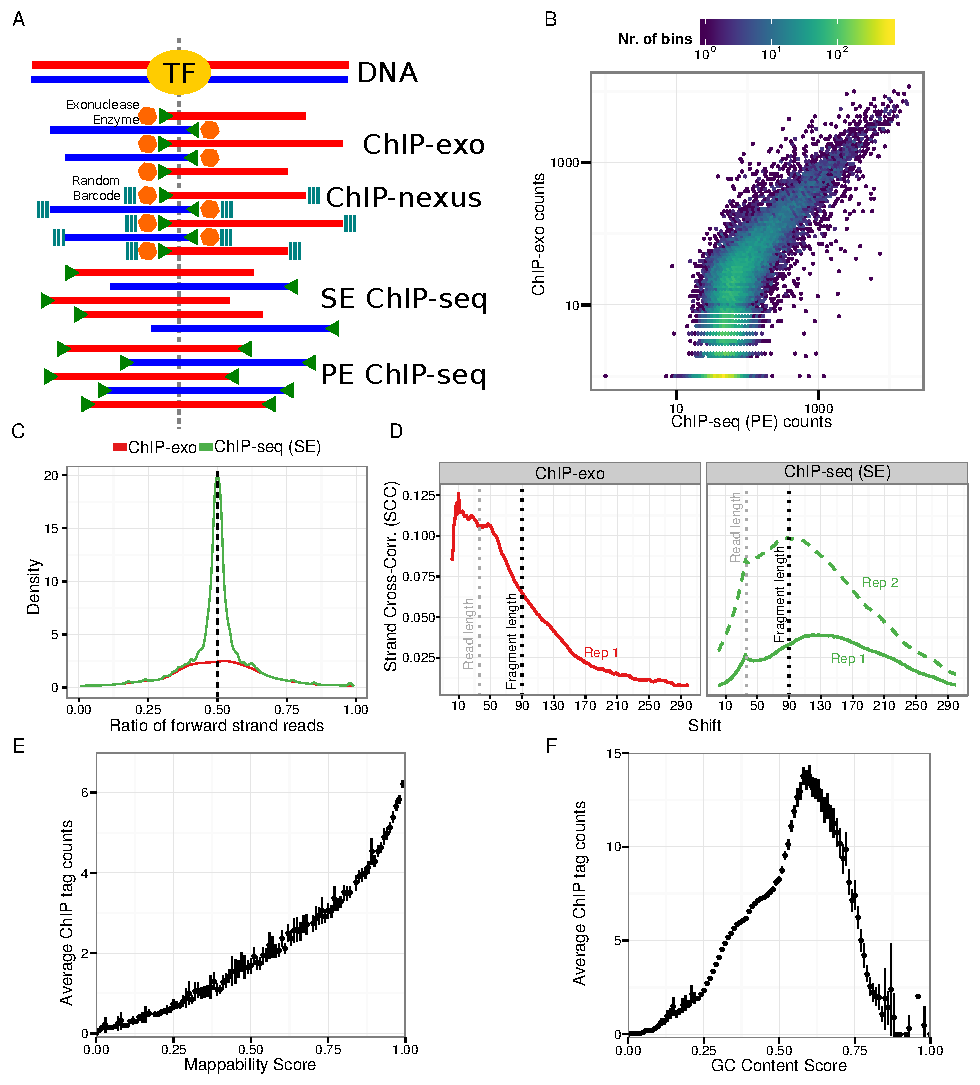
\includegraphics[width = .95\textwidth]{figures/fig1/fig1.pdf}
%  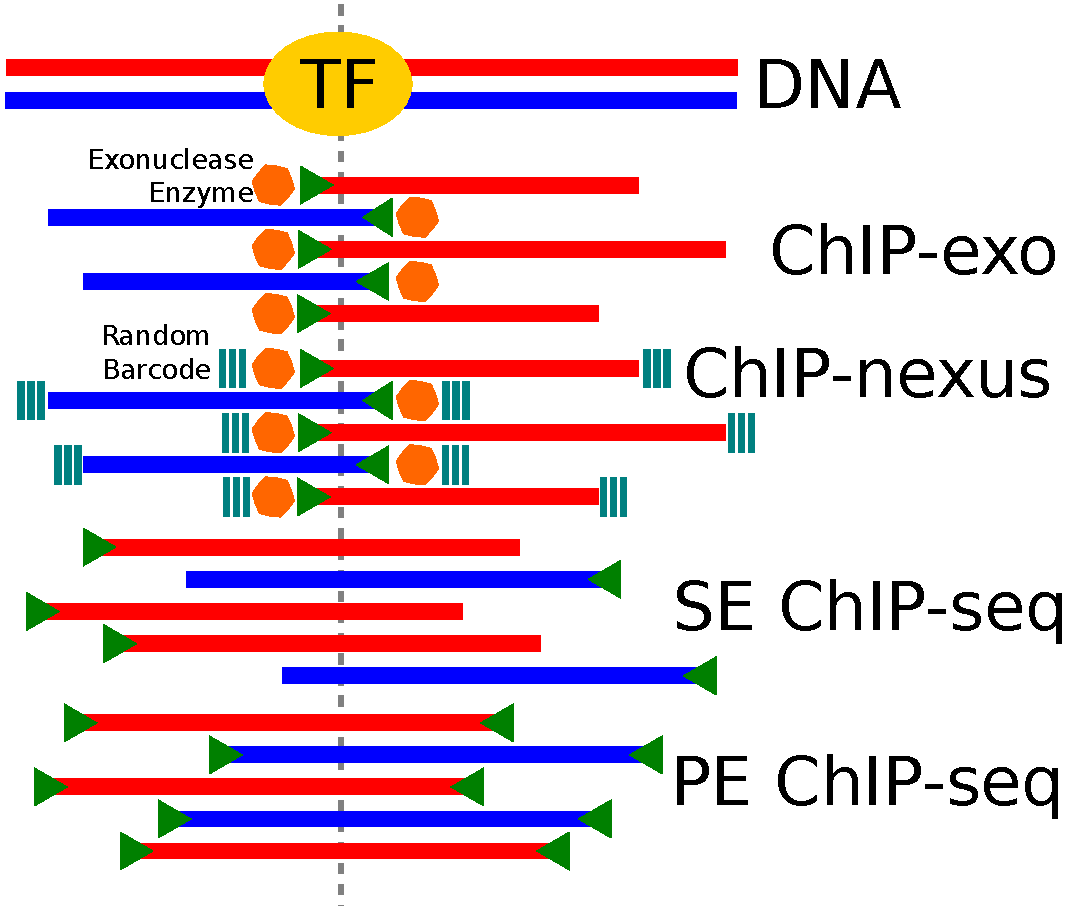
\includegraphics[width =
%  .45 \textwidth]{figures/fig1/chip_explanation_withEnzyme_nexus.pdf}
%  \includegraphics[width = .45\textwidth,page = 3]{figures/fig1/ChIPseqPET_ChIPexo_tagCount_comparison.pdf}
%  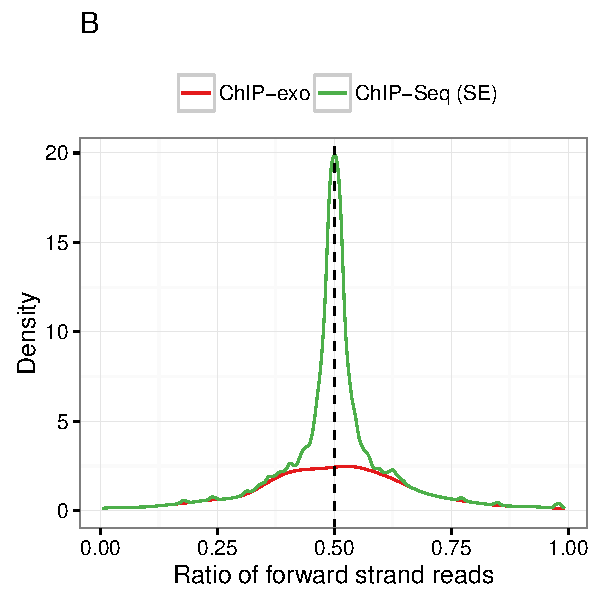
\includegraphics[width =.3\textwidth]{figures/fig1/forward_strand_ratio_comp_old.pdf}
%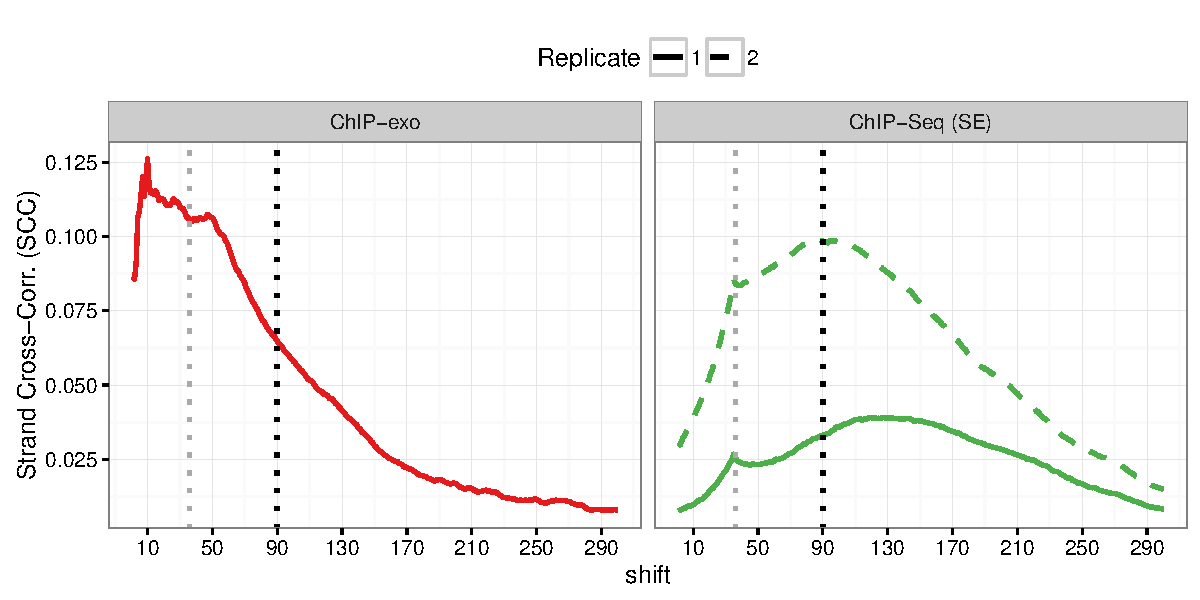
\includegraphics[width = .6 \textwidth]{figures/fig1/scc_ctcf2.pdf}
%  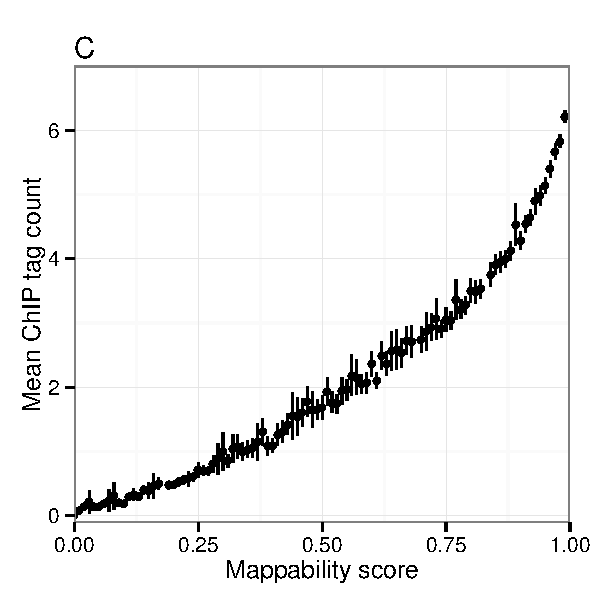
\includegraphics[width = .4\textwidth,page = 1]{figures/fig1/eukaryotic_bias_CTCF.pdf}
%  \includegraphics[width = .4\textwidth,page = 2]{figures/fig1/eukaryotic_bias_CTCF.pdf}
  \caption{A) A TF is bound to the forward (red) and backward (blue)
    strand of the DNA. Then, is sonicated: For ChIP-exo a exonuclease
    enzyme (orange hexagon) trims the $5\prime$ ends of each DNA
    fragment to a fixed distance from the bound protein, finally is
    subjected to Immunoprecipitation and amplification. For ChIP-nexus
    a random barcode is added on the $3\prime$ end, and transferred to
    the $5\prime$ stopping base by self-circularization, after the
    library is amplified and the reads aligned, reads with identical
    barcode and start position are removed. For both ChIP-exo and SE
    ChIP-seq an adapter is ligated (green triangles) at the $5\prime$
    ends, while for PE ChIP-seq is ligated to both ends.  B) Hexbin
    plot of PE ChIP-seq bin counts vs ChIP-exo bin counts. C) Forward
    Strand Ratio densities for SE ChIP-seq and ChIP-exo peaks. D) SCC
    curves for human CTCF on HeLa cell lines.  The SCC curve for the
    ChIP-exo sample from \cite{exo1} is shown in the left panel, and
    the SCC for ChIP-seq samples from \cite{encode1} are shown in the
    right panel. The ChIP-exo curve shows local maxima at the motif
    and read length. Both SE ChIP-seq curves are maximized at the
    fragments length and show a local maxima at its read length. E)
    Mappability score vs mean ChIP tag counts with 0.95 confidence
    bands. F) GC - content score vs mean ChIP tag counts with 0.95
    confidence bands.}
  \label{fig:1}
\end{figure}

    % \textbf{https://www.encodeproject.org/experiments/ENCSR000AOA/}


\newpage

% figure 2

\begin{figure}[h!]
  \centering
  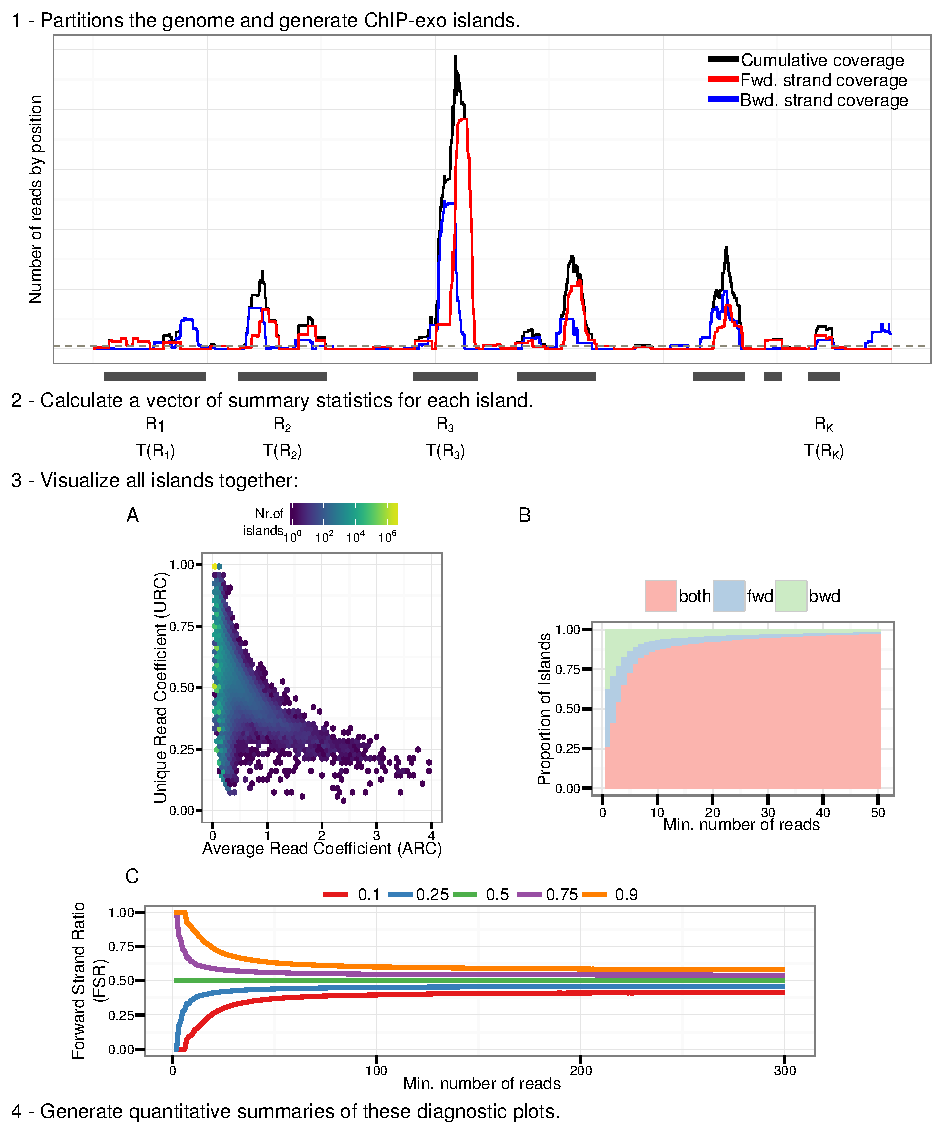
\includegraphics[width = .95\textwidth]{figures/fig2/fig2.pdf}
  \caption{\RW{The ChIP-exo reads are partitioned by keeping the
      regions in the genome composed by the undigested fragments. For
      each region the following summary statistics are calculated:
      Average Read Coefficient (ARC), Unique Read Coefficient (URC)
      and Forward Strand Ratio (FSR). These statistics are visualized
      as: A) ARC vs. URC plots, which presents the overall balance
      between library complexity and enrichment; there are two arms,
      one with low ARC, that corresponds to regions formed by few
      aligned positions and one where the URC decreases as the ARC
      increases, that corresponds to potentially enriched regions. B)
      Region Composition plot, which shows the strand composition for
      all the regions formed by a min. number of reads; low depth
      regions are commonly formed by undigested reads in one unique
      strand, while high depth regions are usually formed by reads in
      both. C) FSR distribution plot, it illustrates the FSR's
      distribution as as higher depth regions are being considered: In
      a high quality experiment the FSR's distribution is tightly
      centered around the FSR's median.}}

  % There are two arms: First, one with low ARC, which corresponds to
  % regions formed by few aligned positions; Second, where the URC
  % decreases as the ARC increases.

  % Regions with low depth tend to be formed by undigested reads from
  % one unique strand, while regions with higher signal are usually
  % formed by reads in both strands.

  % In a high quality sample, the median is around 0.5, and the other
  % quantiles reach that value quickly.
  \label{fig:2}
\end{figure}

\newpage

% figure 3

\begin{figure}[h!]
  \centering
%  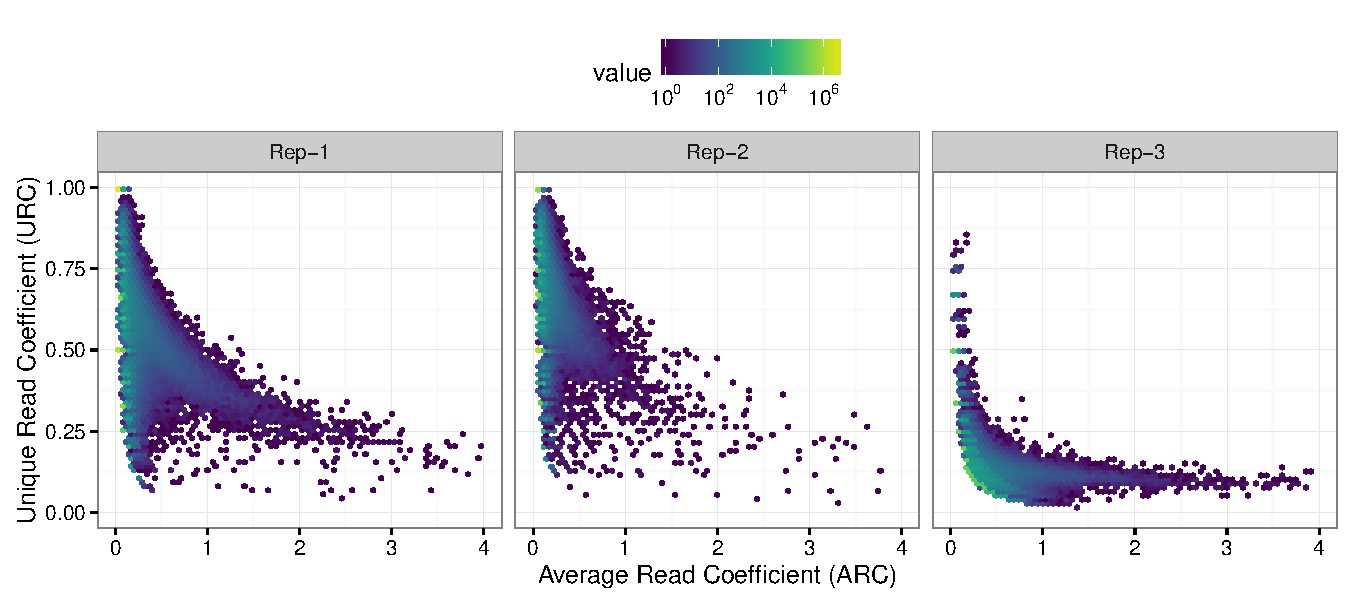
\includegraphics[width = .8\textwidth,page = 1]{figures/fig3/Carroll_FoxA1_mouse_enrichment.pdf}
%  \includegraphics[width = .8\textwidth,page = 3]{figures/fig3/Carroll_FoxA1_mouse_strand_imbalance.pdf} 
%  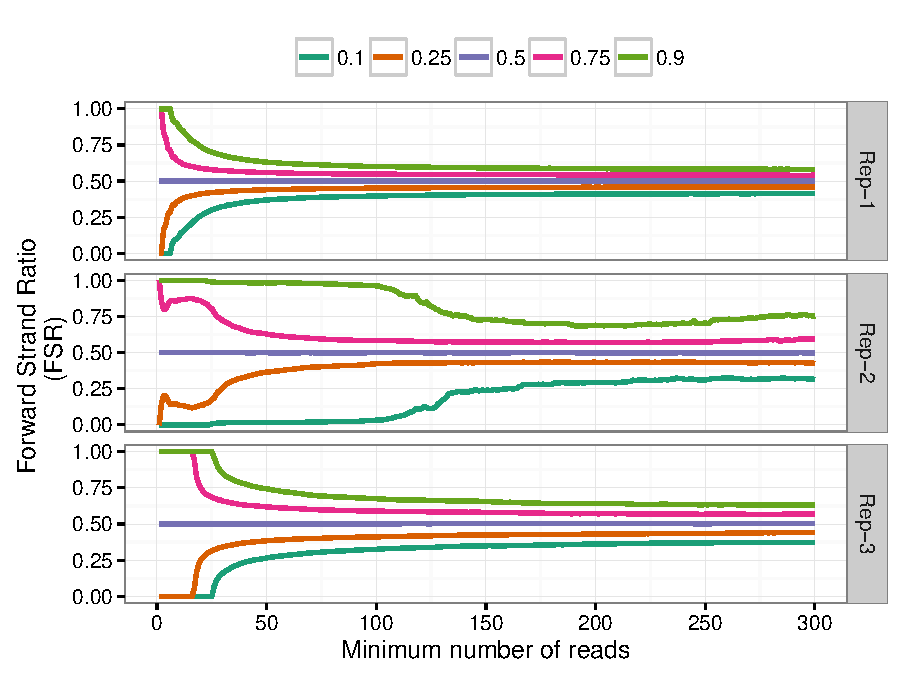
\includegraphics[width = .8\textwidth,page = 1]{figures/fig3/Carroll_FoxA1_mouse_strand_imbalance.pdf} 
    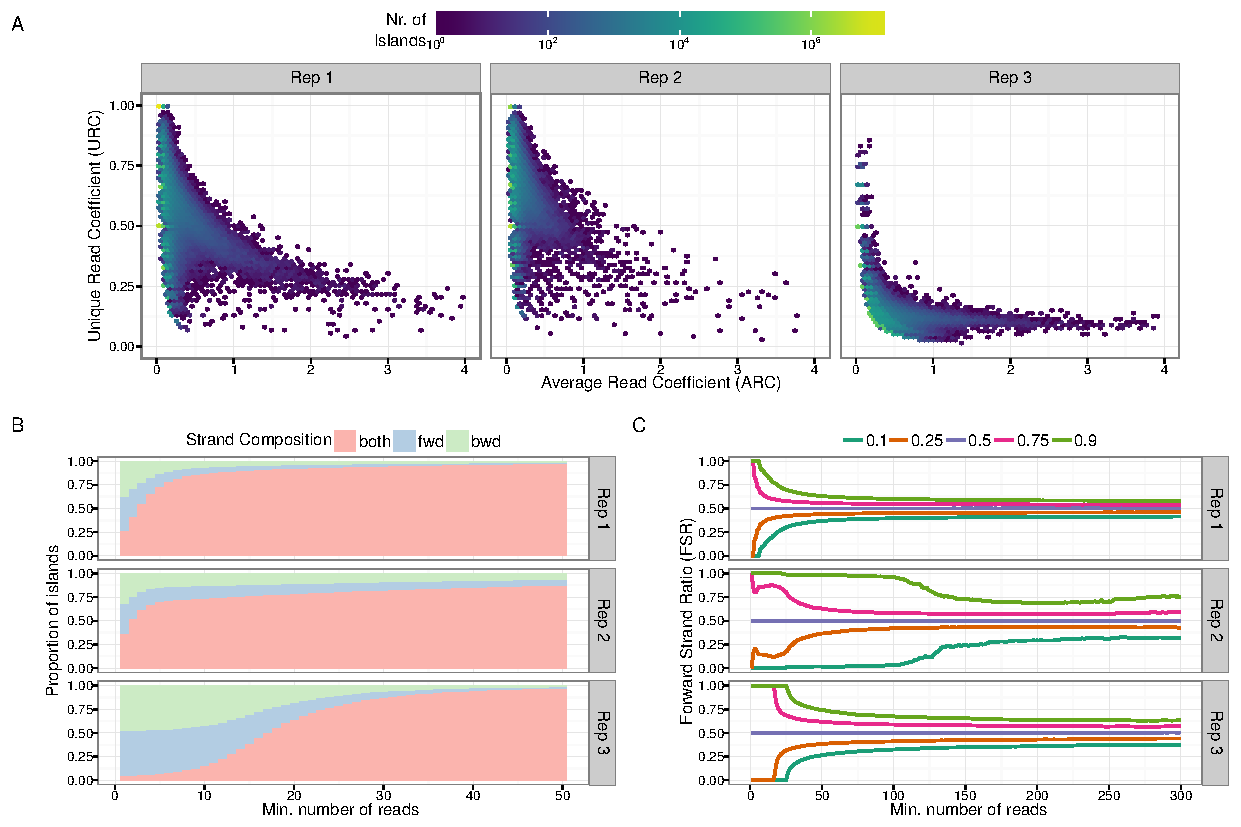
\includegraphics[width = .95\textwidth]{figures/fig3/fig3.pdf}
  \caption{\RW{Diagnostic plots generated by \pname{}. Comparison of
      A) ARC vs. URC plot, B) Region Composition plot and C) FSR
      distribution plot between the three FoxA1 replicates in mouse
      liver tissue from \cite{exoillumina}.}}
  \label{fig:3}
\end{figure}

\newpage

% , there is a slight separation into two strong arms, one corresponds
% to low $\mbox{ARC}$ and varying $\mbox{URCR}$, and for the other
% $\mbox{URCR}$ decreases as $\mbox{ARC}$ increases

%     , all quantiles approach to the median as the lower bound
%     increases

%     , in a good sample the single-stranded regions are going to be
%     filtered out quickly as in the middle row.

\newpage

% figure 4

\begin{figure}[h!]
  \centering  
%  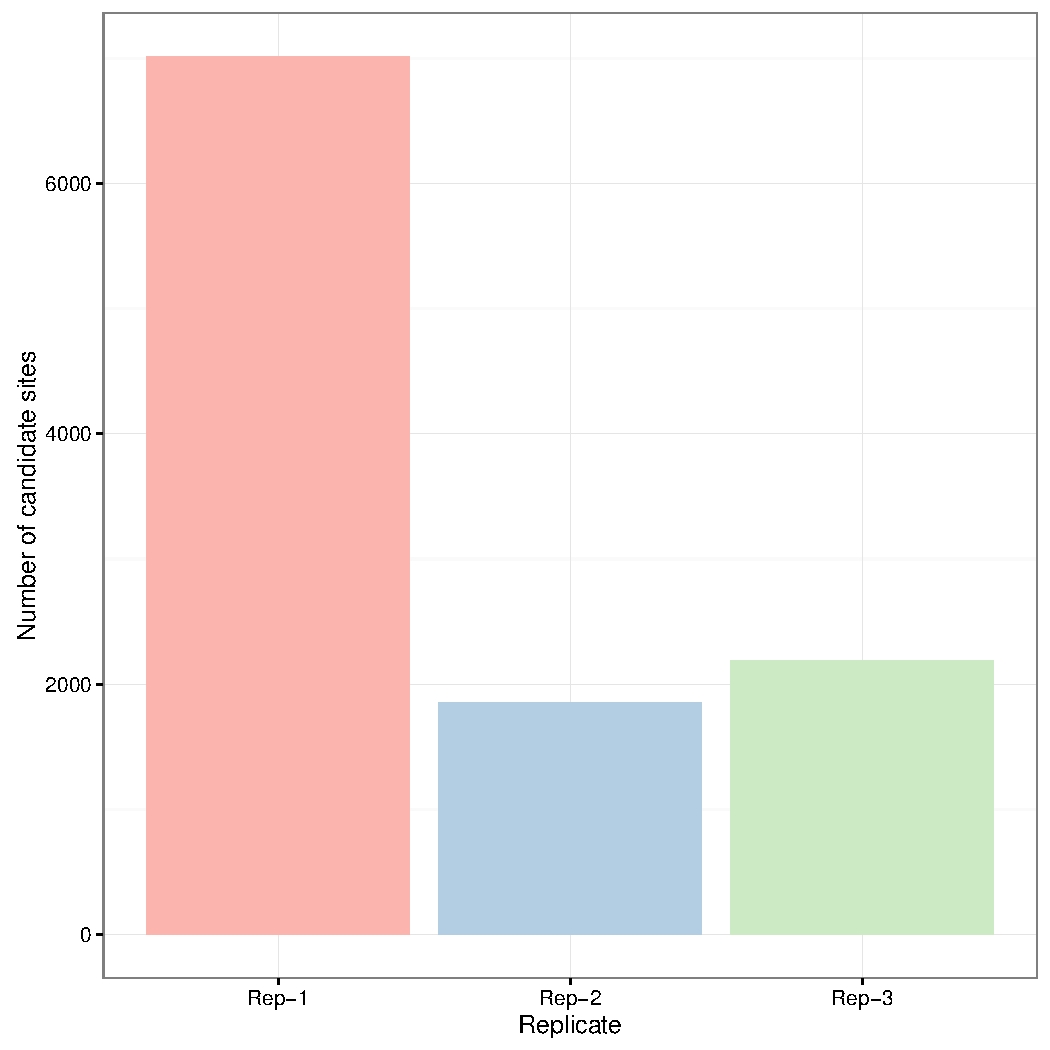
\includegraphics[width = .23 \textwidth, page = 1]{figures/fig4/FoxA1_barplots.pdf}
  \includegraphics[width = .23 \textwidth, page = 3]{figures/fig4/FoxA1_barplots.pdf}
  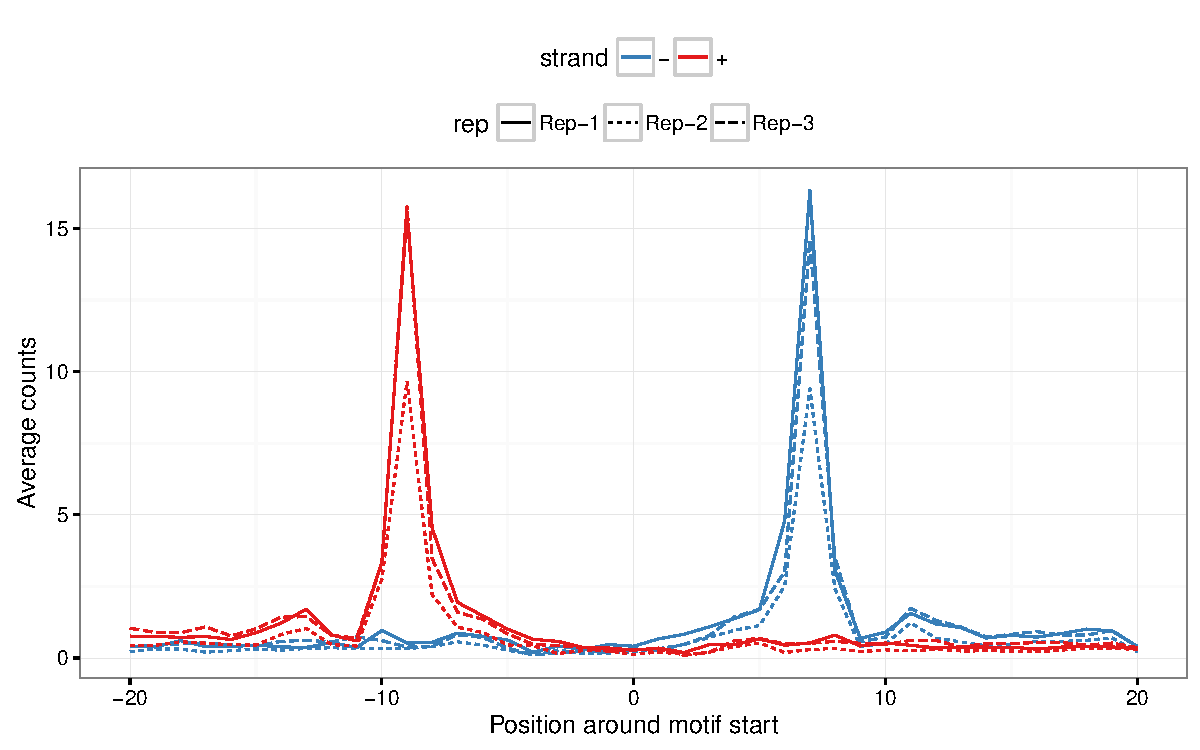
\includegraphics[width =.4\textwidth]{figures/fig4/FoxA1_profiles_around_motif.pdf}
%  \includegraphics[width = .25\textwidth,page = 2]{figures/fig4/FoxA1_matched_motif_sequence.pdf}
%  \includegraphics[width = .25\textwidth,page = 3]{figures/fig4/FoxA1_matched_motif_sequence.pdf}
%  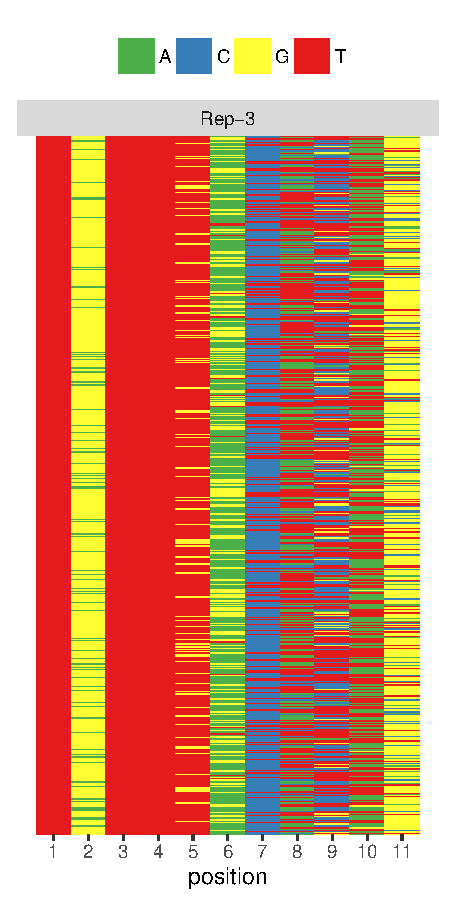
\includegraphics[width = .25\textwidth,page = 1]{figures/fig4/FoxA1_matched_motif_sequence.pdf}  
  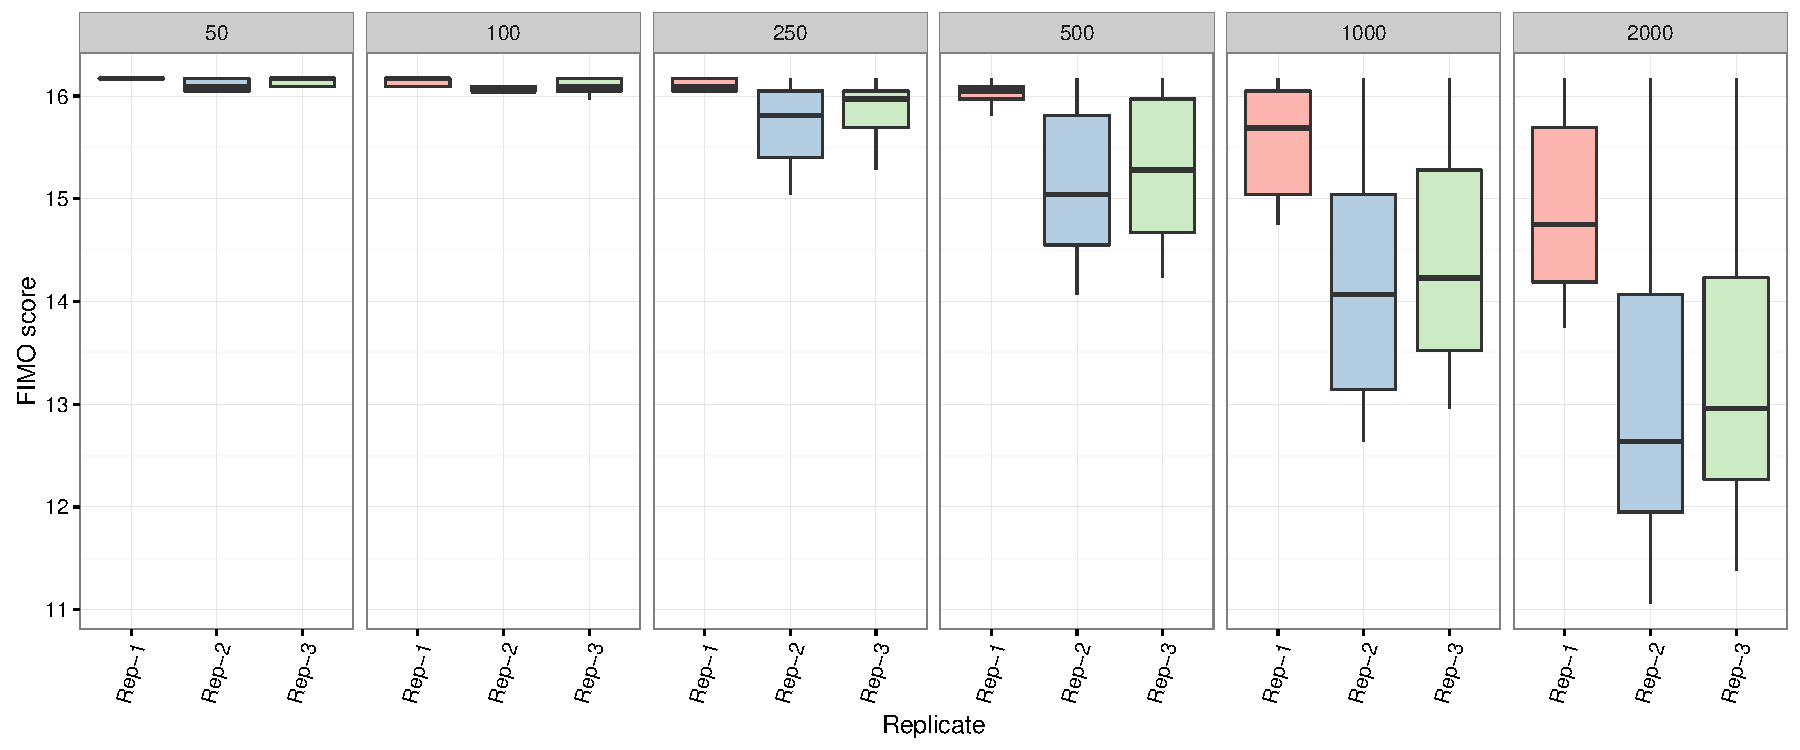
\includegraphics[width = .8\textwidth,page = 1]{figures/fig4/FoxA1_fimo_score.pdf}
  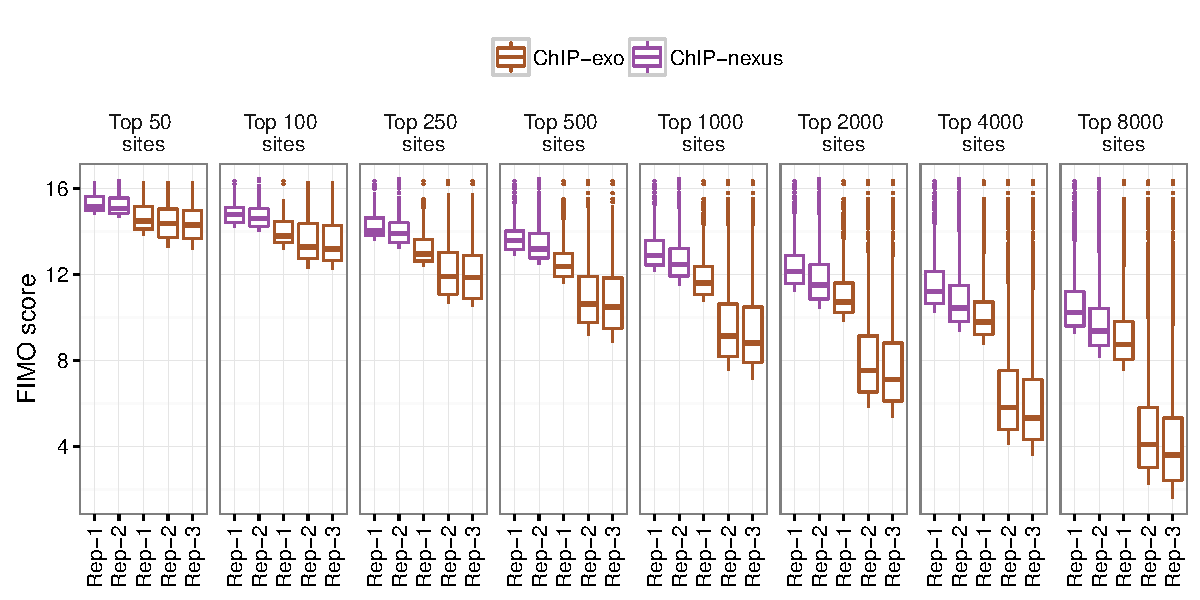
\includegraphics[width = .5\textwidth]{figures/fig4/TBP_scores_comparison.pdf}
%  \includegraphics[width = .8\textwidth,page = 2]{figures/fig4/strand_imbalance_FoxA1.pdf}
  \caption{Using the mouse FoxA1 experiment from \cite{exoillumina}
    and the FoxA1 motif with MA0148.1 id in the \texttt{JASPAR}
    database: \RW{ A) Number of high quality regions where the FoxA1
      motif was searched. B) Proportion of candidate regions with
      motif. C) FoxA1 Average Coverage plots centered around motif
      start positions separated by replicate and strand. D) Sequence
      composition of sites with motif for each replicate. E)
      Comparison of the top 50, 100, 250, 500, 1000 and 2000 FIMO
      scores for each replicate. F) Strand Imbalance comparison of
      regions with at least 50, 100, 150 and 250 reads overlapping
      with ChIP-exo peaks for each replicate.}}
% Strand imbalance using the mouse FoxA1 experiment from
%     \cite{exoillumina}:  C)
%     $-\log_{10}(\text{p.value})$ of testing if the imbalance
%     distributions differs when ChIP-exo regions overlap their peaks.}
  \label{fig:4}
\end{figure}

 % B) Number of
 %    candidate sites for each replicate. C) Percentage of candidate
 %    sites where the FoxA1 motif was detected. D) Average coverage
 %    around FoxA1 motif. Base distribution for matched sequence for
 %    Rep-1 (E), Rep-2 (F) and Rep-3 (G).

\newpage

% figure 5

\begin{figure}[h!]
  \centering
  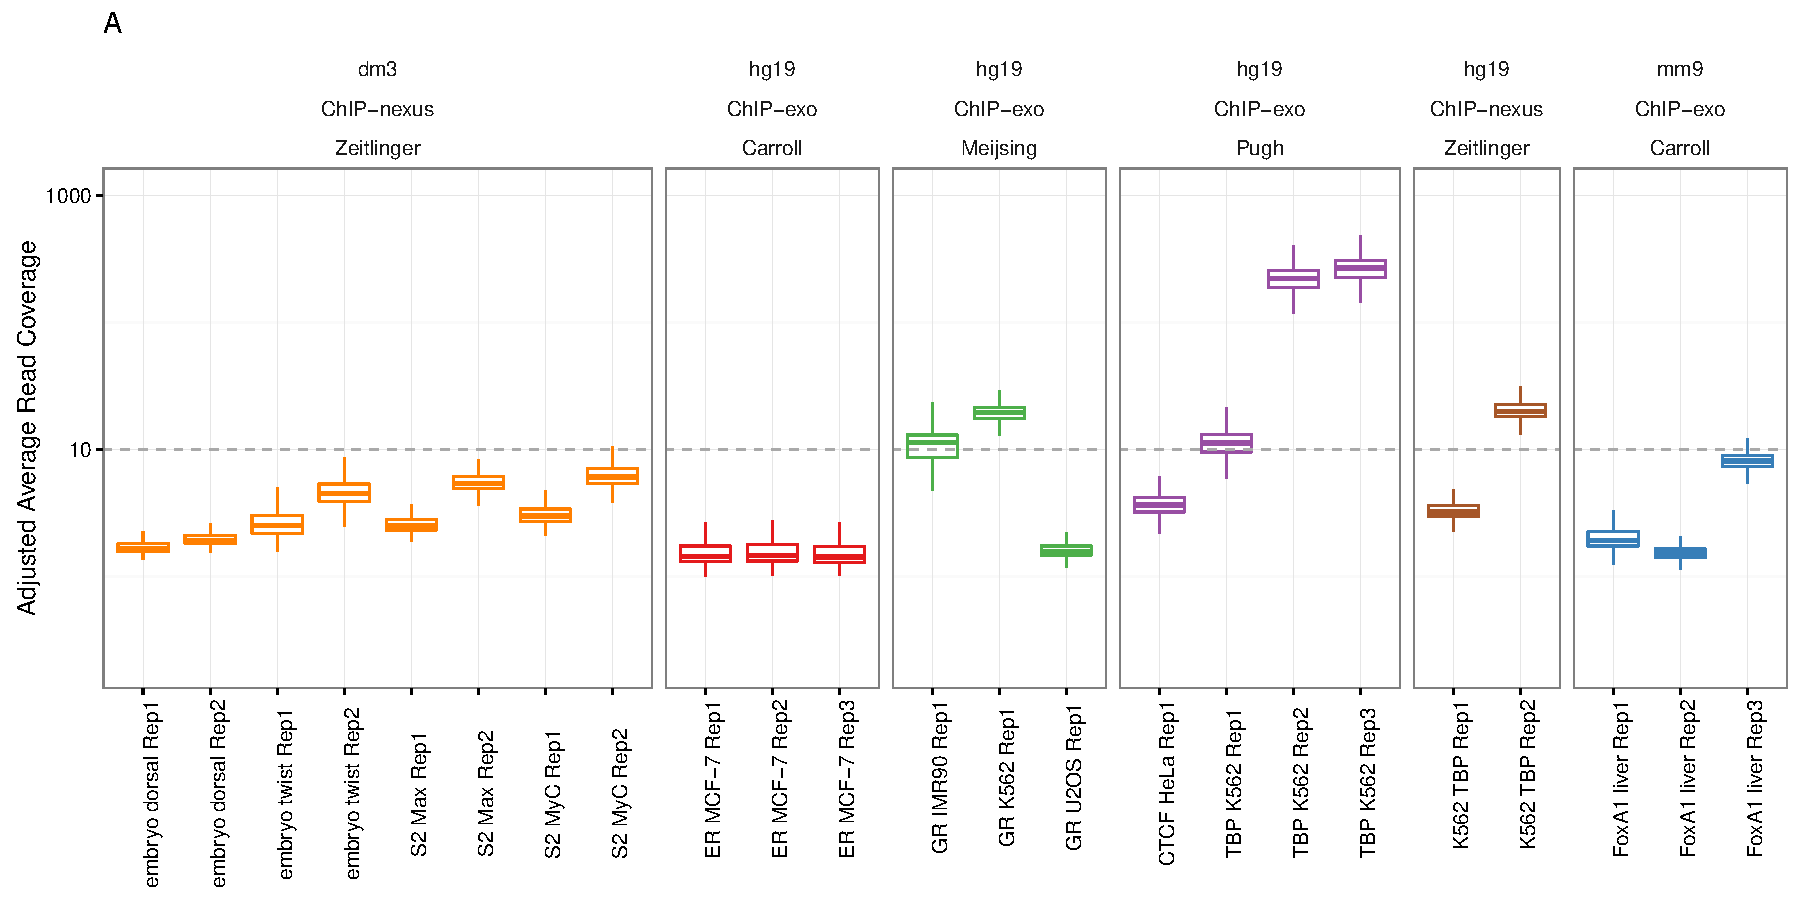
\includegraphics[width = .9  \textwidth,page = 1]{figures/fig5/QC_pipeline_eval_boxplot.pdf}
\newline
  \includegraphics[width = .9  \textwidth,page = 2]{figures/fig5/QC_pipeline_eval_boxplot.pdf}
\newline
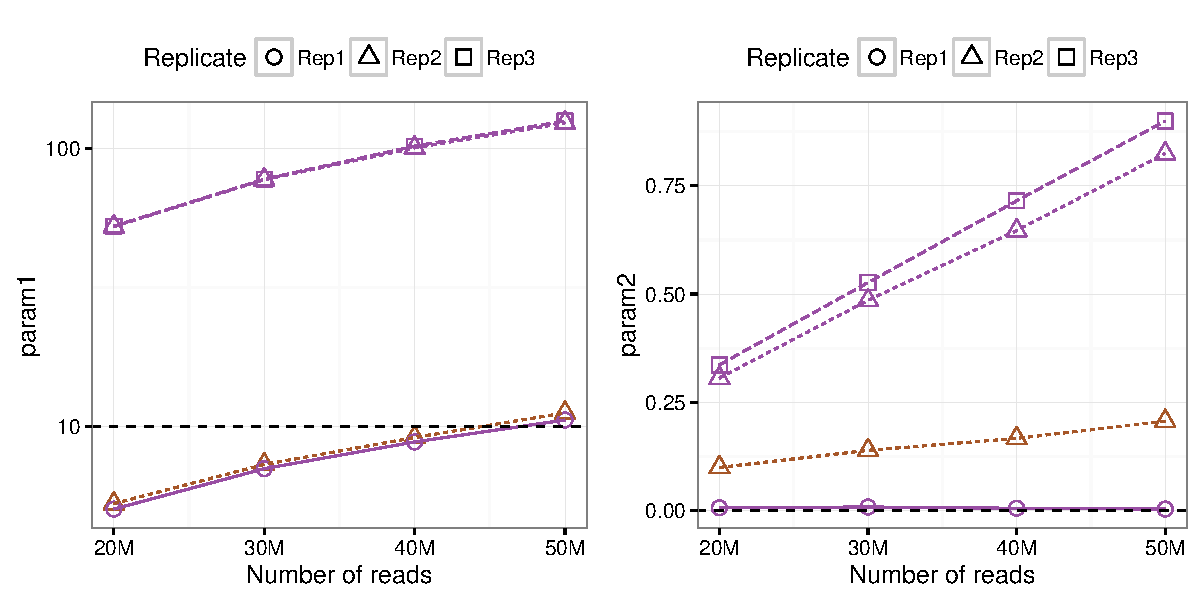
\includegraphics[width = .45\textwidth,page = 1]{figures/fig5/TBP_param_depth_trend.pdf}
  % 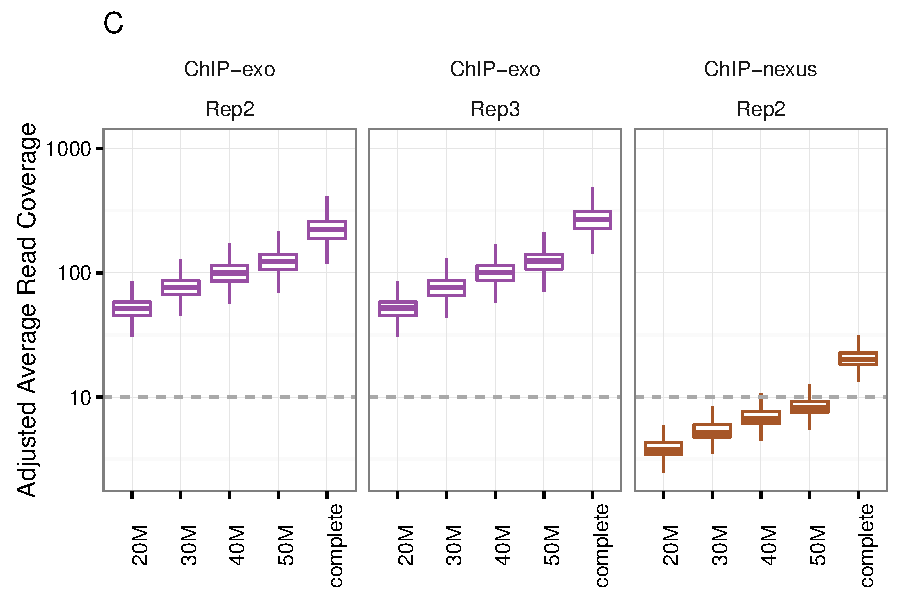
\includegraphics[width = .45  \textwidth,page = 1]{figures/fig5/K562_TBP_sample.pdf}
  % \includegraphics[width = .45  \textwidth,page = 2]{figures/fig5/K562_TBP_sample.pdf}
\caption{\RW{Comparison of all estimated A) $\beta_1$ and B) $\beta_2$
    for all eukaryotic ChIP-exo/nexus samples. Comparison of the
    average estimated A) $\beta_1$ and B) $\beta_2$ for the
    ChIP-exo/nexus TBP samples in K562 cell lines when sub-sampling
    20M to 50M reads. E) Comparison of the top 50, 100, 250, 500,
    1000, 2000, 4000 and 8000 FIMO scores for each TBP experiment. The
    scores were calculated with the TBP MA0108.1 motif in the
    \texttt{JASPAR} database.}}
% \caption{Comparison of adjusted Average Read Coverage and $\mbox{ARC}$
%   bias for eukaryotic genome ChIP-exo and ChIP-nexus experiment. A)
%   Boxplot of adjusted $\mbox{ARC}$. B) Boxplot of large sequencing
%   depth $\mbox{ARC}$'s bias. Comparison of sub-sampled ChIP-exo and
%   ChIP-nexus experiments of TBP factor in human K562 cell lines: C)
%   Adjusted $\mbox{ARC}$ and D) $\mbox{ARC}$'s bias. E) FIMO scores of
%   TBP ChIP-exo and ChIP-nexus samples for best motif scores.}
  \label{fig:5}
\end{figure}

\newpage

% figure 6

\begin{figure}[h!]
  \centering
  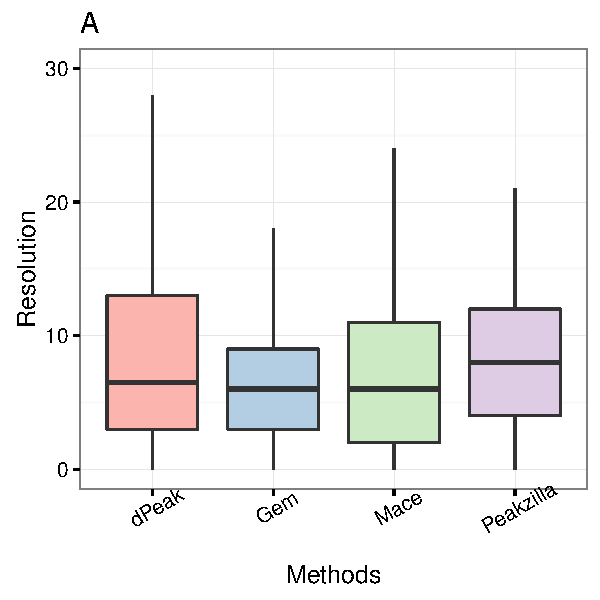
\includegraphics[width = .45\textwidth,page = 1]{figures/fig6/methods_comp_FDR5_topM400.pdf}
  \includegraphics[width = .45\textwidth,page = 2]{figures/fig6/methods_comp_FDR5_topM400.pdf}
   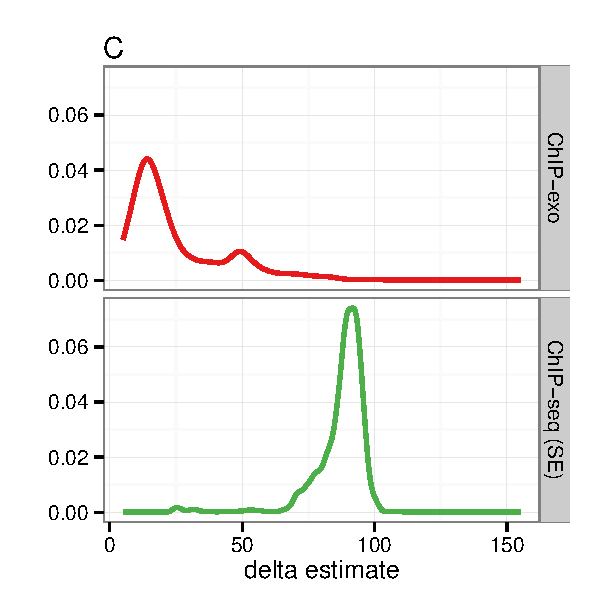
\includegraphics[width = .45\textwidth,page = 1]{figures/fig6/sigma_delta_old_densities.pdf}
   \includegraphics[width = .45\textwidth,page = 2]{figures/fig6/sigma_delta_old_densities.pdf}   
   \caption{\RW{Resolution comparison between dPeak, Gem, Mace and
       Peakzilla using the A) E1-1 and B) E1-2 \textit{E.coli}
       ChIP-exo experiments. Estimated C) $\delta$ and D) $\sigma$
       parameter densities for ChIP-exo (E1-2 sample) and SE ChIP-seq
       (S1-1 sample).}}
% Resolution is the defined as the distance
%        between a RegulonDB annotation and the closest predicted
%        binding event. 
  % \caption{Comparison of the resolution between dPeak, Gem, Mace and
  %   Peakzilla methods with \emph{E.Coli} aerobic experiment from the
  %   first biosample A) Replicate 1 and B) Replicate 2. Resolution is
  %   defined as the minimum distance between a RegulonDB annotation and
  %   a predicted binding event. C) $\delta$ parameter in dPeak measures
  %   average distance of the reads to their respective binding site. In
  %   ChIP-exo data, reads were located much closer to the binding site
  %   than in SET ChIP-Seq. D) $\sigma$ parameter measure the dispersion
  %   of reads around each binding site. In ChIP-exo data, reads showed
  %   less variation around the their respective binding sites compared
  %   to SET ChIP-Seq.}
  \label{fig:6}
\end{figure}

\newpage

% figure 7
% \RW{For now, I kept the next two figures separated. If we decide to
%   include the analysis of Fig8 in the main text, then I consider we
%   should merge both into fig 7. ChIP-exo depths is rougly the half of
%   PE ChIP-seq which may work into our advantage since we are obtaining
%   comparable resolution and better sensitivity with less reads. On the
%   other hand, the SE ChIP-seq depth is roughly the half from the
%   ChIP-exo making that comparison a little bit unfair (which may not
%   be a big deal since the other comparison is the most important
%   one).}

\begin{figure}[h]
  \centering
  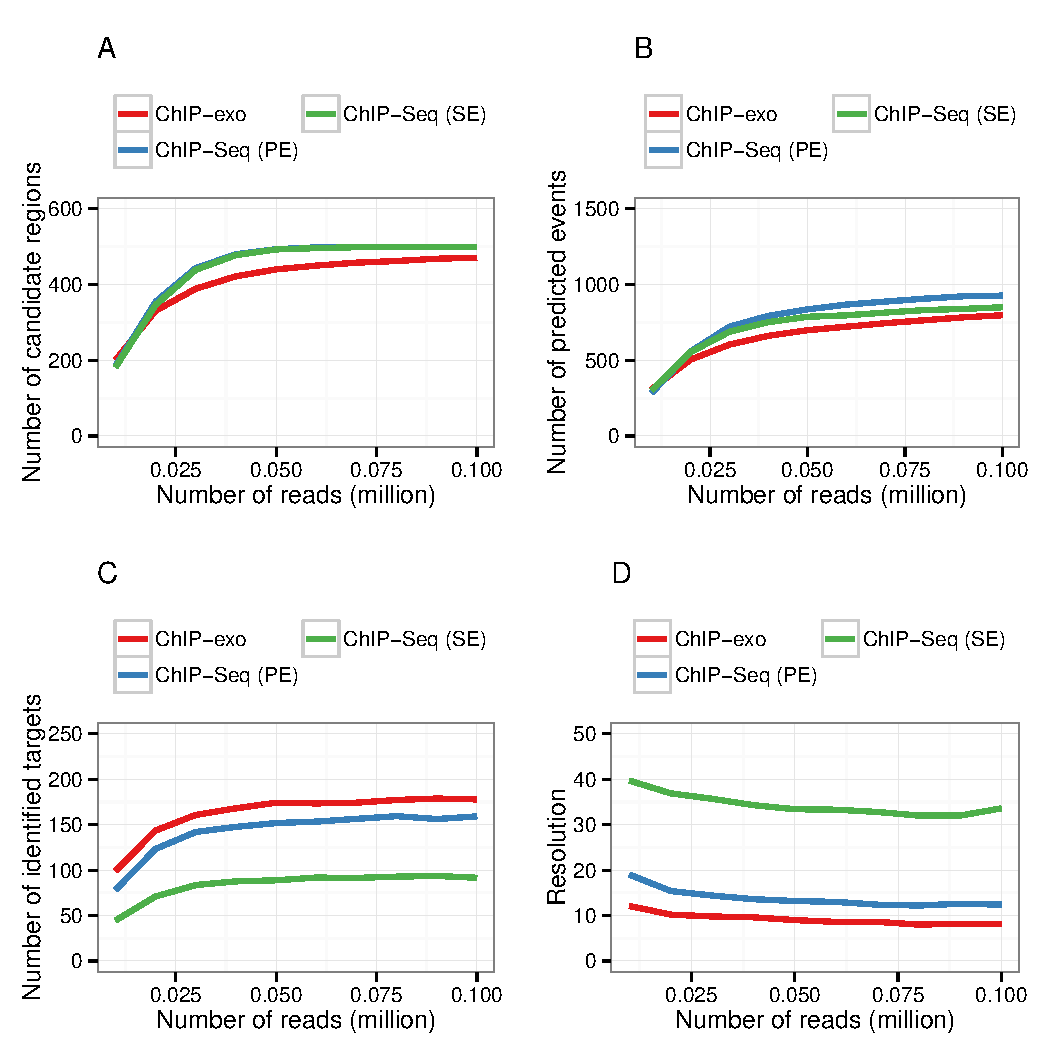
\includegraphics[width = .9\textwidth]{figures/fig7/saturation_analysis_old.pdf}
  \caption{Comparison of the number of A) candidate regions, B)
    predicted events, C) identified targets and D) resolution among
    ChIP-exo, PE ChIP-seq and SE ChIP-seq.}
 % A RegulonDB binding event
 %    was deemed identified if a binding event was estimated at a $\pm$
 %    15 vicinity of it.
  \label{fig:7}
\end{figure}

% figure 8

\begin{figure}[h!]
  \centering
  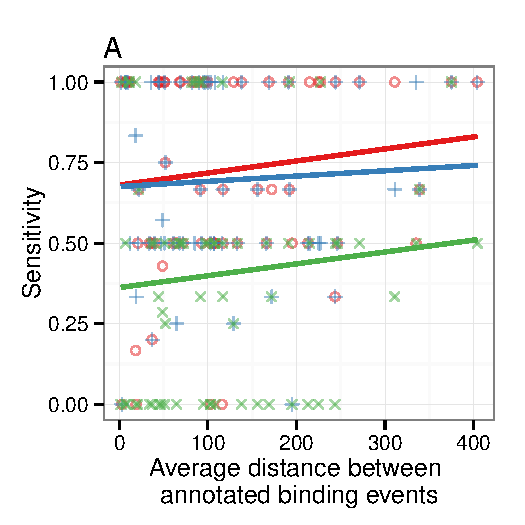
\includegraphics[width = .46\textwidth]{figures/fig8/sensitivity_exo_olda_data.pdf}
  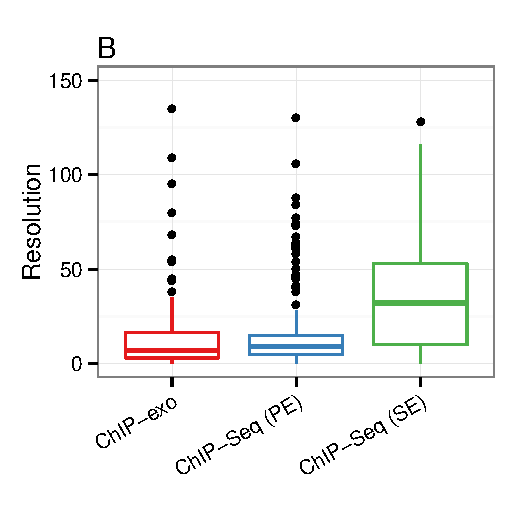
\includegraphics[width = .46\textwidth]{figures/fig8/resolution_by_dataset_old_data.pdf}
  \caption{Comparison of A) sensitivity and B) resolution between
    ChIP-exo and ChIP-seq data.}
  % Sensitivity is defined as the proportion of RegulonDB annotations
  % identified using each data. Resolution is defined as the distance
  % between RegulonDB annotation and its closest prediction.
  \label{fig:8}
\end{figure}


\end{document}


% LocalWords:  Ntimes overlaping gaussian repk depts
